\documentclass{article}

\usepackage{../../util}

\title{Differential Equations}
\author{Cambridge University Mathematical Tripos: Part IA}

\begin{document}
\maketitle

\tableofcontentsnewpage{}

\section{Differentiation and orders of magnitude}
The Differential Equations course is all about the mathematics of how things change.

\subsection{Introduction}
\begin{definition}[Differential Equation]
	A differential equation (DE) is an equation involving derivatives of a function or several functions.
\end{definition}
\begin{definition}[Limit, informally]
	If \(\lim\limits_{x \to x_0} f(x) = A\), then \(f(x)\) can be made arbitrarily close to \(A\) by making \(x\) sufficiently close to \(x_0\).
\end{definition}
Note that the definition of the limit does not specify behaviour of \(f(x)\) at \(x=x_0\); it is perfectly possible that \(f(x_0)\) is undefined, or that it is some number not equal to \(A\).
Examples of this behaviour would be \(1/x\) (undefined at 0), or the Dirac \(\delta\) function (infinite at 0).

\begin{definition}[One-Sided Limit]
	A left limit is notated \(\lim\limits_{x \to x_0^-}\).
	It requires that the value \(A\) represented by the limit is computed by setting \(x\) to values smaller than \(x_0\).
	Analogously, a right limit is notated \(\lim\limits_{x \to x_0^+}\).
	In calculating this limit, \(x\) must be greater than \(x_0\).
\end{definition}

\begin{wrapfigure}{l}{0.5\textwidth}
	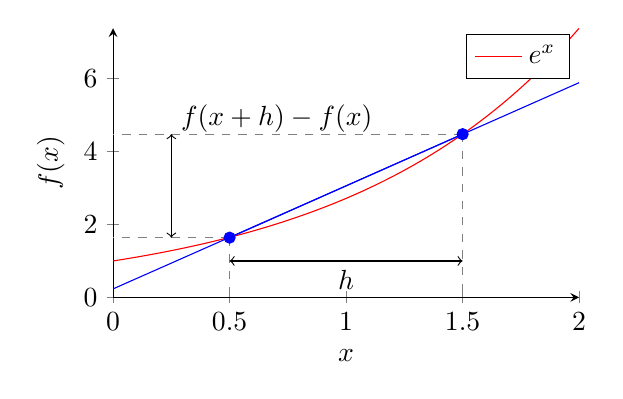
\begin{tikzpicture}
		\begin{axis}[
				axis lines = left,
				xlabel = \(x\),
				ylabel = {\(f(x)\)},
				width=7.5cm,
				height=5cm,
				xmin=0,
				ymin=0
			]

			\addplot [
				domain=0:2,
				samples=100,
				color=red,
			]
			{e^x};
			\addlegendentry{\(e^x\)}

			\addplot [
				domain=0:2,
				samples=100,
				color=blue,
			]
			{2.83*(x-0.5) + e^0.5};

			\addplot [
				color=blue,
				mark=*,
			]
			coordinates {
					(0.5, 1.64) (1.5,4.48)
				};

			\draw [dashed,gray] (axis cs:0.5,1.64) -- (axis cs:0.5,0);
			\draw [dashed,gray] (axis cs:1.5,4.48) -- (axis cs:1.5,0);
			\draw [dashed,gray] (axis cs:0.5,1.64) -- (axis cs:0,1.64);
			\draw [dashed,gray] (axis cs:1.5,4.48) -- (axis cs:0,4.48);

			\draw [<->] (axis cs:0.5,1) -- node [below]{\(h\)} (axis cs:1.5,1);
			\draw [<->] (axis cs:0.25,1.64) -- node [right,yshift=0.85cm]{\(f(x+h)-f(x)\)} (axis cs:0.25,4.48);
		\end{axis}
	\end{tikzpicture}
\end{wrapfigure}

\begin{definition}[Derivative]
	We can use the definitions of limits to define the derivative of a function \(f(x)\) with respect to its argument (in this case, \(x\)):
	\begin{equation}\label{derivative}
		\frac{\dd{f}}{\dd{x}} = \lim_{h \to 0} \frac{f(x+h)-f(x)}{h}
	\end{equation}
\end{definition}

Pictorially, we can see that the definition of the derivative is basically the slope of the line between two points that approach arbitrarily close to each other.
In this example, \(x\) is 0.5, and \(h\) is 1.

Note that for the derivative to exist at a point \(x\), we require that

\[
	\lim_{h \to 0^-} \frac{f(x+h)-f(x)}{h} = \lim_{h \to 0^+} \frac{f(x+h)-f(x)}{h}
\]

This excludes, for example, the derivative of \(\abs{x}\) at \(x=0\), as this would have two conflicting answers (\(-1\) and 1).

\subsection{Notation}
There are multiple ways of representing derivatives of functions.
Here, we show the derivative of \(f(x)\) in multiple notation systems:
\begin{itemize}
	\item \(\displaystyle \frac{\dd{f}}{\dd{x}}\): Leibniz notation
	\item \(f'(x)\): Lagrange notation
	\item \(\dot f (x)\): Newton notation
\end{itemize}

For sufficiently smooth functions (meaning that the derivative is valid at each step), we can define derivatives recursively:
\[
	\frac{\ddempty}{\dd{x}}\left( \frac{\dd{f}}{\dd{x}} \right)
	= \frac{\dn 2 f}{\dd{x}^2}
	= f''(x) = \ddot f (x)
\]

\subsection{Rules for differentiation}
\begin{definition}[Chain Rule]
	Consider a function \(f(x) = F(g(x))\).
	The derivative of \(f(x)\) can be written
	\begin{equation}
		\frac{\dd{f}}{\dd{x}} = F'(g(x)) \cdot g'(x) = \frac{\dd{F}}{\dd{g}} \frac{\dd{g}}{\dd{x}}
	\end{equation}
\end{definition}

\begin{definition}[Product Rule]
	Consider a function \(f(x) = u(x)v(x)\).
	The derivative of \(f(x)\) can be written
	\begin{equation}
		\frac{\dd{f}}{\dd{x}} = u'(x)v(x) + u(x)v'(x) = u'v + uv'
	\end{equation}
\end{definition}

\begin{definition}[Leibniz' Rule]
	Consider a function \(f(x) = u(x)v(x)\).
	Recursive derivatives of \(f(x)\) can be written
	\begin{align}
		f    & = uv                                        \\
		f'   & = u'v + uv' \nonumber                       \\
		f''  & = u''v + 2u'v' + uv'' \nonumber             \\
		f''' & = u'''v + 3u''v' + 3u'v'' + uv''' \nonumber
	\end{align}
	This is analogous to Pascal's triangle and the binomial expansion.
	The coefficients are \(n!/m!(n-m)!
	\), more often written \(n \choose m\).
\end{definition}

\subsection{Order of magnitude}
The goal of `order of magnitude' functions is to compare the size of functions in the vicinity of certain points.
\begin{definition}[Little \(o\)]
	Given functions \(f(x)\) and \(g(x)\) such that
	\begin{equation}
		\lim\limits_{x \to x_0} \frac{f(x)}{g(x)} = 0
	\end{equation}
	we can say that \(f(x) = o(g(x))\) as \(x \to x_0\).
\end{definition}

This is essentially saying that the function \(f(x)\) is much `smaller' than \(g(x)\) as we approach the point \(x_0\).
For example, \(x^2 = o(x)\) as \(x \to 0\), because \(x^2\) becomes vanishingly small compared to \(x\) near zero.

\begin{definition}[Big \(O\): \(x_0\) finite]
	Assume we have two functions \(f(x)\) and \(g(x)\), and a finite number \(x_0\) where we are comparing the functions.
	If we can find two positive constants \(M\) and \(\delta\) such that
	\begin{equation}
		\abs{f(x)} \leq M\abs{g(x)} \quad(\forall x,\, \abs{x-x_0} < \delta)
	\end{equation}
	then \(f(x) = O(g(x))\) as \(x \to x_0\).
\end{definition}
Informally, the function \(f\) can be \textit{bounded by} \(g\) in a specific area around the point \(x_0\).

Unlike little \(o\) notation, there is no requirement that \(f(x)\) becomes vanishingly small compared to \(g(x)\), just that it is smaller.
Therefore, \(x^2 \neq o(x^2)\) but \(x^2 = O(x^2)\) (both as \(x \to 0\)).

Some examples:
\begin{itemize}
	\item \(x^2 = O(x)\) as \(x \to 0\).
	      Take \(M = 1\), \(\delta = 1\).
	\item \(x \neq O(x^2)\) as \(x \to 0\).
	      This is because for any value of \(x\) smaller than \(1/M\), the value of \(g(x)\) is \(Mx^2\) which is smaller than \(x\).
	\item \(x^2 = O(x^2)\) as \(x \to 0\).
	      Take \(M = 1\), and choose an arbitrary \(\delta\).
\end{itemize}

By convention, we usually pick the most restrictive \(M\) and \(\delta\) possible.

\begin{definition}[Big \(O\): \(x_0\) infinite]
	Assume we have two functions \(f(x)\) and \(g(x)\), and we want to compare the functions' behaviours at infinity.
	If we can find two positive constants \(M\) and \(x_1\) such that
	\begin{equation}\label{bigoinf}
		\abs{f(x)} \leq M\abs{g(x)} \quad(\forall x > x_1)
	\end{equation}
	then \(f(x) = O(g(x))\) as \(x \to \infty\).
\end{definition}

This is basically the same as the previous definition --- but obviously we can't pick a value slightly less than infinity to test, so we just provide a lower bound on \(x\) where the condition holds true.

For example, \(2x^3 + 4x + 12 = O(x^3)\) as \(x \to \infty\).
This is because the function is a cubic, so can be bounded by a cubic as it shoots off to infinity.
We can take, for example, \(M = 3\) and \(x_1 = 3\).
Note that we can't just pick \(M=2\) even though asymptotically the function is close to \(2x^3\); there is a value added to the \(2x^3\) so we'd need to pick a slightly larger number to guarantee that Equation \eqref{bigoinf} is satisfied.

\subsection{Equation of a tangent}
We can use little \(o\) notation to construct the equation of a tangent to a function \(f(x)\) at a given \(x\) value, \(x_0\).
This is the start of the formula for the Taylor series of \(f\) at \(x_0\).

First, notice that \(o(g(x))/g(x)\) is zero, as \(o(g(x))\) is vanishingly small compared to \(g(x)\) near the convergence point.

Using Equation \eqref{derivative}, we can (informally) deduce:

\begin{align*}
	\eval{\frac{\dd{f}}{\dd{x}}}_{x=x_0} & = \frac{f(x_0 + h) - f(x_0)}{h}                          \\
	                                     & = \frac{f(x_0 + h) - f(x_0)}{h} + \frac{o(h)}{h}         \\
	\therefore f(x_0 + h)                & = f(x_0) + \eval{\frac{\dd{f}}{\dd{x}}}_{x=x_0} h + o(h)
\end{align*}
If we now take \(x=x_0+h;\,y=f(x);\,y_0=f(x_0)\), we have
\[
	y = y_0 + \eval{\frac{\dd{f}}{\dd{x}}}_{x=x_0}(x - x_0) + o(h)
\]
This is the equation of the tangent to the curve at \(x_0\) if \(o(h)=0\), and this is start of the equation for the Taylor series.

\section{Taylor series and l'H\^opital's rule}
\subsection{Taylor series}
Suppose that we want to approximate a function \(f(x)\) using a polynomial of order \(n\).
\[
	f(x) \approx \underbrace{a_0 + a_1 x + a_2 x^2 + \cdots + a_n x^n}_{\mathclap{\equiv p_n(x)}}
\]
By assuming that the equality holds, we may set \(x=0\) to get the value of \(a_0\).
By differentiating the left and right hand sides \(k\) times, we can evaluate both sides at \(x=0\) to get the value of \(a_k\).
Therefore, term \(a_k\) is equivalent to \(f^{(k)}(0)/k!
\)
\[
	f(x) \approx p_n(x) = f(0) + xf'(0) + \frac{x^2}{2}f''(0) + \cdots + \frac{x^n}{n!}f^{(n)}(0)
\]
Alternatively, repeating the process at \(x_0\), we get the formula for the Taylor polynomial of degree \(n\) of \(f(x)\):
\[
	f(x) \approx p_n(x) = f(x_0) + (x-x_0)f'(x_0) + \frac{(x-x_0)^2}{2}f''(x_0) + \cdots + \frac{(x-x_0)^n}{n!}f^{(n)}(x_0)
\]
We can write
\begin{equation}\label{taylorerror}
	f(x) = p_n(x) + E_n
\end{equation}
where \(E_n\) is the error at term \(n\).
Recall that \(f(x+h) = f(x) + hf'(x) + o(h)\) as \(h \to 0\).
We can generalise this, provided that the first \(n\) derivatives of \(f(x)\) exist.
\begin{equation}\label{xplush}
	f(x+h) = f(x) + hf'(x) + \frac{h^2}{2}f''(x) + \cdots + \frac{h^n}{n!}f^{(n)}(x) + o(h^n)
\end{equation}
Comparing Equations \eqref{taylorerror} and \eqref{xplush}, we see that:
\[
	E_n = o(h^n)
\]
\begin{theorem}[Taylor's Theorem]
	\(E_n = O(h^{n+1})\) as \(h \to 0\) provided that \(f^{(n+1)}(x)\) exists.
\end{theorem}
Note that the big \(O\) notation in Taylor's Theorem is a stronger statement than the little \(o\) notation above.
For example, \(h^{n+a}=o(h^n)\) as \(h \to 0\ \forall a \in (0, 1)\) since \(\lim_{h\to 0} \frac{h^n+a}{h^n} = \lim_{h\to 0} h^a = 0\).
However, \(h^{n+a} \neq O(h^{n+1})\) as \(h \to 0\) for \(a \in (0, 1)\) because we can't bound \(h^{n+a}\) using \(h^{n+1}\) everywhere in the vicinity of \(0\).

\subsection{L'H\^opital's rule}
Let \(f(x)\) and \(g(x)\) be differentiable functions at \(x=x_0\), and that \(\lim_{x\to x_0} f(x) = f(x_0) = 0\) and similarly for \(g(x)\).
L'H\^opital's Rule states that
\[
	\lim_{x\to x_0} \frac{f(x)}{g(x)} = \lim_{x\to x_0} \frac{f'(x)}{g'(x)} \text{ if } g'(x_0) \neq 0
\]
\begin{proof}
	As \(x \to x_0\):
	\begin{align*}
		f(x)              & = f(x_0) + (x-x_0) f'(x_0) + o(x-x_0)                                       \\
		g(x)              & = g(x_0) + (x-x_0) g'(x_0) + o(x-x_0)                                       \\
		\intertext{But we know that \(f(x_0)=g(x_0)=0\) therefore}
		\frac{f(x)}{g(x)} & = \frac{f'(x_0) + \frac{o(x-x_0)}{x-x_0}}{g'(x_0) + \frac{o(x-x_0)}{x-x_0}} \\
		\intertext{By the definition of little \(o\), \(o(h)/h\) tends to zero, so}
		\frac{f(x)}{g(x)} & = \frac{f'(x)}{g'(x)}
	\end{align*}
\end{proof}
Note that l'H\^opital's rule can be applied recursively, using higher-order derivatives.
For example, consider \(f(x) = 3\sin x - \sin 3x\); \(g(x) = 2x - \sin 2x\).
The limit approaches 3 as \(x \to 0\).

\section{Integration}
\subsection{Definition of integration}
We use a Riemann sum to approximate the area under a sufficiently well-behaved function \(f(x)\) on the real numbers.
\begin{equation}\label{riemannsum}
	\sum_{n=0}^{N-1} f(x_n) \Delta x
\end{equation}
where \(\Delta x = (b-a)/N\), and \(x_n = a + n\Delta x\).
How close is \eqref{riemannsum} to the area under \(f(x)\) for large \(N\)?
Consider a specific rectangle in the Riemann sum by fixing \(n\).
The area under the curve in the \(n\)th rectangle and the area of the rectangle itself differ by a value we denote here as \(\varepsilon\).
By computing \(\varepsilon\)'s order of magnitude, we can show how much the total error deviates by.

\begin{theorem}[Mean Value Theorem]
	For a continuous function \(f(x)\),
	\begin{equation}\label{meanvaluetheorem}
		\int_{x_n}^{x_{n+1}} f(x) \dd{x} = f(x_c) \cdot (x_{n+1} - x_n)
	\end{equation}
	for some \(x_c\in (x_n, n_{n+1})\).
\end{theorem}
\noindent We use the Taylor Series of \(f(x)\) at \(x_n\) to compute a value for \(x_c\).
\[
	f(x_c) = f(x_n) + O(x_c - x_n)
\]
as \(x_c - x_n \to 0\).
Since \(x_n < x_c < x_{n+1}\), which implies \(\abs{x_{n+1} - x_n} > \abs{x_c - x_n}\), we can make the statement that
\[
	f(x_c) = f(x_n) + O(x_{n+1} - x_n)
\]
as \(x_{n+1} - x_n \to 0\).
Thus, by \eqref{meanvaluetheorem}
\[
	\int_{x_n}^{x_{n+1}} f(x) \dd{x} = \left[ f(x_n) + O(x_{n+1} - x_n) \right] (x_{n+1} - x_n)
\]
By defining \(\Delta x = x_{n+1} - x_n\), we have
\begin{equation}
	\int_{x_n}^{x_{n+1}} f(x) \dd{x} = \Delta x f(x_n) + O(\Delta x ^ 2)
\end{equation}
By rearranging, we can compute \(\varepsilon\):
\[
	\varepsilon = \abs{\int_{x_n}^{x_{n+1}} f(x) \dd{x} - \Delta x f(x_n)} = O(\Delta x ^ 2)
\]
Therefore it follows that
\[
	\int_{a}^{b} f(x) \dd{x} = \lim_{\Delta x \to 0} \left[ \left( \sum_{n=0}^{N-1} f(x_n) \Delta x \right) + O(N\Delta x^2) \right]
\]
Note that \(O(N\Delta x^2) = O((\frac{b-a}{N})^2 \cdot N) = O(1/N)\), so
\[
	\int_{a}^{b} f(x) \dd{x} = \lim_{N \to \infty} \left[ \left( \sum_{n=0}^{N-1} f(x_n) \Delta x \right) + O(1/N) \right]
\]
Which gives our final result of
\begin{equation}\label{definiteintegral}
	\int_{a}^{b} f(x) \dd{x} = \lim_{N \to \infty} \sum_{n=0}^{N-1} f(x_n) \Delta x
\end{equation}

\subsection{Fundamental theorem of calculus}
Let \(F(x) = \int_{a}^{x} f(t) \dd{t}\).
From the definition of the derivative, we have
\begin{align*}
	\frac{\dd{F}}{\dd{x}} & = \lim_{h \to 0} \frac{1}{h} \left[ F(x+h) - F(x) \right]                                         \\
	                      & = \lim_{h \to 0} \frac{1}{h} \left[ \int_{a}^{x+h} f(t) \dd{t} - \int_{a}^{x} f(t) \dd{t} \right] \\
	                      & = \lim_{h \to 0} \frac{1}{h} \int_{x}^{x+h} f(t) \dd{t}                                           \\
	\intertext{Using \eqref{definiteintegral}:}
	                      & = \lim_{h \to 0} \frac{1}{h} \left[ hf(x) + O(h^2) \right]                                        \\
	                      & = \lim_{h \to 0} \left[ f(x) + O(h) \right]                                                       \\
	                      & = f(x)
\end{align*}
Therefore:
\begin{equation}\label{ftc}
	\frac{\ddempty}{\dd{x}} \left[ \int_{a}^{x} f(t) \dd{t} \right] = f(x)
\end{equation}

\subsection{Integration techniques}
Three particularly important methods of integration are:
\begin{itemize}
	\item \(u\)-substitution,
	\item trigonometric substitutions, and
	\item integration by parts.
\end{itemize}
Of particular note is the trigonometric substitution method, since it can be difficult to work out exactly which substitution will yield the result.
A table is provided below.

\begin{center}
	\begin{tabular}{c c c}
		Identity                              & Term in Integrand  & Substitution        \\\midrule
		\(\cos^2 \theta + \sin^2 \theta = 1\) & \(\sqrt{1 - x^2}\) & \(x = \sin \theta\) \\
		\(1 + \tan^2 \theta = \sec^2 \theta\) & \(1 + x^2\)        & \(x = \tan \theta\) \\
		\(\cosh^2 u - \sinh^2 u = 1\)         & \(\sqrt{x^2 - 1}\) & \(x = \cosh u\)     \\
		\(\cosh^2 u - \sinh^2 u = 1\)         & \(\sqrt{x^2 + 1}\) & \(x = \sinh u\)     \\
		\(1 - \tanh^2 u = \sech^2 u\)         & \(1 - x^2\)        & \(x = \tanh u\)
	\end{tabular}
\end{center}

\section{Multivariate functions}
\subsection{Partial derivatives}
We define the partial derivative of a two-valued function \(f(x, y)\) with respect to \(x\) (for example) by:
\begin{equation}
	\eval{\frac{\partial f}{\partial x}}_{y} = \lim_{\delta x\to 0} \frac{f(x + \delta x, y) - f(x, y)}{\delta x}
\end{equation}
For example, if \(f(x,y) = x^2 + y^3 + e^{xy^2}\), we have
\begin{align*}
	\eval{\frac{\partial f}{\partial x}}_{y}     & = 2x + y^2 e^{xy^2} \\
	\eval{\frac{\partial^2 f}{\partial x^2}}_{y} & = 2 + y^4 e^{xy^2}
\end{align*}
We can also define `cross-derivatives' by differentiating successively with respect to different variables, for example
\[
	\eval{\frac{\partial}{\partial y} \left( \eval{\frac{\partial f}{\partial x}}_{y} \right)}_{x} = 2ye^{xy^2} + 2xy^3e^{xy^2}
\]
The order of computation of cross-derivatives is irrelevant, provided that the required derivatives all exist.
\begin{equation}
	\frac{\partial^2 f}{\partial x \partial y} = \frac{\partial}{\partial x}\frac{\partial f}{\partial y} = \frac{\partial}{\partial y}\frac{\partial f}{\partial x} = \frac{\partial^2 f}{\partial y \partial x}
\end{equation}
We use a subscript shorthand to denote partial differentiation.
Where the point of evaluation of the derivative is not stated, it is implied to be fixed.
For example:
\[
	\eval{\frac{\partial f}{\partial x}}_{y} = \frac{\partial f}{\partial x} = f_x
\]
However, with a function \(f(x, y, z)\):
\[
	\eval{\frac{\partial f}{\partial x}}_{yz} \neq \eval{\frac{\partial f}{\partial x}}_{y}
\]
because \(z\) is not fixed.

\subsection{Multivariate chain rule}
In this section, all use of \(o\) notation is defined to be where all required \(\delta\) values approach 0.
We define the differential of a two-valued function \(f(x, y)\) to be
\begin{equation}\label{differential}
	\delta f = f(x + \delta x, y + \delta y) - f(x, y)
\end{equation}
We can evaluate this differential by rewriting \eqref{differential} as
\begin{align*}
	\delta f =\  & f(x + \delta x, y + \delta y) - f(x + \delta x, y)\ + \\
	             & f(x + \delta x, y) - f(x, y)
\end{align*}
We can move from \((x, y)\) to \((x + \delta x, y + \delta y)\) along the path \((x, y) \to (x + \delta x, y) \to (x + \delta x, y + \delta y)\).
If we move in this way, then we only need to worry about derivatives in the directions of our axes.
From here on in the derivation, the first line will always represent the path segment in the \(y\) direction, and the second line will represent the path segment in the \(x\) direction.

Now that we've separated the differential into these two axes, we can use Taylor series, treating each line as a single-valued function, to expand each of these path segments along the matching axis.
\begin{align*}
	\delta f =\  & f(x + \delta x, y) + \delta y\frac{\partial f}{\partial y}(x + \delta x, y) + o(\delta y) - f(x + \delta x, y)\ + \\
	             & f(x, y) + \delta x \frac{\partial f}{\partial x}(x, y) + o(\delta x) - f(x, y)
\end{align*}
We can now cancel the beginning and ending points of each segment of the path, leaving
\begin{align*}
	\delta f =\  & \delta y\frac{\partial f}{\partial y}(x + \delta x, y)\ + o(\delta y)+ \\
	             & \delta x \frac{\partial f}{\partial x}(x, y) + o(\delta x)
\end{align*}
We can reduce the remaining \(x+\delta x\) term to simply an \(x\) term by performing another Taylor expansion.
\begin{align*}
	\delta f =\  & \delta y\left[ \frac{\partial f}{\partial y}(x, y) + \delta x\frac{\partial^2 f}{\partial y^2}(x, y) + o(\delta x) \right] + o(\delta y)\ + \\
	             & \delta x \frac{\partial f}{\partial x}(x, y) + o(\delta x)
\end{align*}
Expanding out this bracket leaves
\begin{align*}
	\delta f =\  & \delta y\frac{\partial f}{\partial y}(x, y) + \delta x\delta y\frac{\partial^2 f}{\partial y^2}(x, y) + o(\delta x \delta y) + o(\delta y)\ + \\
	             & \delta x \frac{\partial f}{\partial x}(x, y) + o(\delta x)
\end{align*}
We will now change the meanings of each line.
Now, we will group terms by factors.
\begin{align*}
	\delta f =\  & \delta x \frac{\partial f}{\partial x}(x, y) + o(\delta x)\ +                  \\
	             & \delta y\frac{\partial f}{\partial y}(x, y) + o(\delta y)\ +                   \\
	             & \delta x\delta y\frac{\partial^2 f}{\partial y^2}(x, y) + o(\delta x \delta y)
\end{align*}
Because \(o(h)\) is significantly smaller than \(h\), we can eliminate all the \(o\) terms.
\begin{align*}
	\delta f =\  & \delta x \frac{\partial f}{\partial x}(x, y)\ +         \\
	             & \delta y\frac{\partial f}{\partial y}(x, y)\ +          \\
	             & \delta x\delta y\frac{\partial^2 f}{\partial y^2}(x, y)
\end{align*}
Finally, we can eliminate the \(\delta x \delta y\) term because it is vanishingly small as they tend to zero.
\begin{equation}
	\delta f = \delta x \frac{\partial f}{\partial x}(x, y) +
	\delta y\frac{\partial f}{\partial y}(x, y)
\end{equation}
This is the differential form of the multivariate chain rule.
We can take the result of this equation in the limit to create the infinitesimal form:
\begin{equation}\label{mvcr}
	\dd{f} = \dd{x} \frac{\partial f}{\partial x}(x, y) +
	\dd{y}\frac{\partial f}{\partial y}(x, y)
\end{equation}

\subsection{Integral form of multivariate chain rule}
By integrating \eqref{mvcr}, we get
\[
	\int \dd{f} = \int \frac{\partial f}{\partial x}\ \dd{x} + \int \frac{\partial f}{\partial y}\ \dd{y}
\]
In definite integral form, we can write
\begin{align*}
	f(x_2 - x_1, y_2 - y_1) & = \int_{x_1}^{x_2} \frac{\partial f}{\partial x}(x, y_1)\ \dd{x} + \int_{y_1}^{y_2} \frac{\partial f}{\partial y}(x_2, y)\ \dd{y}    \\
	                        & = \int_{y_1}^{y_2} \frac{\partial f}{\partial y}(x_1, y)\ \dd{y} + \int_{x_1}^{x_2} \frac{\partial f}{\partial x}(x, y_2)\ \dd{x}    \\
	                        & \neq \int_{x_1}^{x_2} \frac{\partial f}{\partial x}(x, y_1)\ \dd{x} + \int_{y_1}^{y_2} \frac{\partial f}{\partial y}(x_1, y)\ \dd{y}
\end{align*}
Note that the first two examples of a right hand side go along the paths \((x_1, y_1) \to (x_2, y_1) \to (x_2, y_2)\) and \((x_1, y_1) \to (x_1, y_2) \to (x_2, y_2)\) by performing the integrals.
However, the last example does not follow a path from \((x_1, y_1)\) to \((x_2, y_2)\), so it is invalid.

\subsection{Change of variables}
We can transform derivatives into different coordinate systems to make problems easier to solve.
For example, let \(f(x, y)\) be some function with a Cartesian coordinate input.
We can rewrite it in terms of polar coordinates \((r, \theta)\).
First, rewrite \(f\) as:
\[
	f(x(r, \theta), y(r, \theta))
\]
then we can write the derivatives.
\[
	\frac{\partial f}{\partial r} = \frac{\partial f}{\partial x}\frac{\partial x}{\partial r} + \frac{\partial f}{\partial y}\frac{\partial y}{\partial r}
\]
We can do similar evaluations for \(\frac{\partial f}{\partial \theta}\), for example.

\subsection{Implicit differentiation}
Consider some surface defined by \(f(x, y, z) = c\).
Then \(f\) implicitly defines functions such as \(z(x, y)\) (provided the function is well-behaved).
We can find, for example, \(\eval{\frac{\partial z}{\partial x}}_y\) by using the multivariate chain rule in three dimensions.

\[
	\eval{\frac{\partial f}{\partial x}}_y =
	\eval{\frac{\partial f}{\partial x}}_{yz} \underbrace{\eval{\frac{\partial x}{\partial x}}_{y}}_{\mathclap{=1}} +
	\eval{\frac{\partial f}{\partial y}}_{xz} \underbrace{\eval{\frac{\partial y}{\partial x}}_{y}}_{\mathclap{=0}} +
	\eval{\frac{\partial f}{\partial z}}_{xy} \eval{\frac{\partial z}{\partial x}}_{y}
\]
Note that the \(\frac{\partial y}{\partial x}\) term is zero because we hold \(y\) to be fixed.
Simplifying, we get
\[
	\eval{\frac{\partial f}{\partial x}}_y =
	\eval{\frac{\partial f}{\partial x}}_{yz} +
	\eval{\frac{\partial f}{\partial z}}_{xy} \eval{\frac{\partial z}{\partial x}}_{y}
\]
The left hand side is zero because on the surface \(z(x, y)\), \(f\) is always equivalent to \(c\) so there is never any \(\delta f\).
The \(\eval{\frac{\partial f}{\partial x}}_{yz}\) term, however, is not zero in general because we are not going across the \(z(x, y)\) surface --- just parallel to the \(x\) axis, because we fixed both \(y\) and \(z\).
Hence,
\[
	\eval{\frac{\partial z}{\partial x}}_y = \frac{-\eval{\frac{\partial f}{\partial x}}_{yz}}{\eval{\frac{\partial f}{\partial z}}_{xy}}
\]

\subsection{Reciprocal rule}
The reciprocal rule for derivatives applies also to partial derivatives so long as the same variables are held fixed.
For example, given the function \(f(x(r, \theta), y(r, \theta))\), we have
\[
	\eval{\frac{\partial r}{\partial x}}_y = \frac{1}{\eval{\frac{\partial x}{\partial r}}_y}
\]
But
\[
	\frac{\partial r}{\partial x} \neq \frac{1}{\frac{\partial x}{\partial r}}
\]
because the left hand side holds \(y\) constant and the right hand side holds \(\theta\) constant.

\subsection{Differentiating an integral with respect to a parameter}
Consider a family of function \(f(x; \alpha)\) where \(\alpha\) is some parameter.
We can say that \(\alpha\) parametrises \(f\).
An example of a parametrised function is the logarithm; \(f(x; \alpha) = \log_\alpha x\).
We define
\[
	I(\alpha) = \int_{a(\alpha)}^{b(\alpha)} f(x; \alpha) \ \dd{x}
\]
So, what is \(\frac{\dd{I}}{\dd \alpha}\)?
By definition, we have
\begin{align*}
	\frac{\dd{I}}{\dd \alpha} & = \lim_{\delta \alpha \to 0} \frac{I(\alpha + \delta \alpha) - I(\alpha)}{\delta \alpha}                                                                                                                                                                                                                                                  \\
	                          & = \lim_{\delta \alpha \to 0} \frac{1}{\delta\alpha} \left[ \int_{a(\alpha + \delta\alpha)}^{b(\alpha + \delta\alpha)} f(x; \alpha + \delta\alpha)\ \dd{x} - \int_{a(\alpha)}^{b(\alpha)} f(x; \alpha)\ \dd{x} \right]                                                                                                                     \\
	                          & = \lim_{\delta \alpha \to 0} \frac{1}{\delta\alpha} \left[ \int_{a(\alpha)}^{b(\alpha)} f(x; \alpha + \delta\alpha) - f(x; \alpha)\ \dd{x} - \int_{a(\alpha)}^{a(\alpha + \delta)} f(x; \alpha + \delta \alpha)\ \dd{x} + \int_{b(\alpha)}^{b(\alpha + \delta)} f(x; \alpha + \delta \alpha)\ \dd{x} \right]                              \\
	                          & = \int_{a(\alpha)}^{b(\alpha)} \lim_{\delta \alpha \to 0} \frac{f(x; \alpha + \delta\alpha) - f(x; \alpha)}{\delta\alpha}\ \dd{x} - f(a; \alpha) \lim_{\delta \alpha \to 0} \frac{a(\alpha + \delta\alpha) - a(\alpha)}{\delta\alpha} + f(b; \alpha) \lim_{\delta \alpha \to 0} \frac{b(\alpha + \delta\alpha) - b(\alpha)}{\delta\alpha} \\
\end{align*}
Therefore:
\[
	\frac{\dd{I}}{\dd \alpha} = \frac{\dd}{\dd \alpha} \int_{a(\alpha)}^{b(\alpha)} f(x; \alpha) \ \dd{x} = \int_{a(\alpha)}^{b(\alpha)} \frac{\partial f}{\partial \alpha} \ \dd{x} + f(b; \alpha) \frac{\dd{b}}{\dd \alpha} - f(a; \alpha) \frac{\dd{a}}{\dd \alpha}
\]

\section{Linear ordinary differential equations}
\subsection{Eigenfunctions}
\begin{definition}
	The eigenfunction of an operator is a function that is unchanged by the action of the operator (except for a multiplicative scaling).
\end{definition}
From this definition, we can see that \(e^{\lambda x}\) is the eigenfunction of the differential operator.
The eigenvalue of this function is \(\lambda\), as this is the scaling factor.

\subsection{Rules for linear ODEs}
\begin{enumerate}
	\item Any linear homogeneous ODE with constant coefficients has solutions in the form \(e^{\lambda x}\).
	      For example, in the equation \(5y' - 3y = 0\) we can try a solution of the form \(y = Ae^{\lambda x}\), and we get \(5 \lambda - 3 = 0\).
	      This equation is known as the characteristic equation.
	\item Any solution to a linear homogeneous ODE can be scaled to create more solutions.
	      In particular, \(y=0\) is a solution.
	\item An \(n\)th order linear ODE has \(n\) linearly independent solutions.
	      In the case of constant coefficient equations, this follows from the Fundamental Theorem of Algebra.
	      However, the proof of this is outside the scope of this course.
	      This implies that the above example has only one solution: \(y = Ae^{3x/5}\).
	\item An \(n\)th order ODE requires \(n\) initial/boundary conditions to create a particular solution.
\end{enumerate}

\subsection{Solving first order ODEs}
To solve a differential equation, we can use the following technique to break it apart into two smaller functions:
\[
	y = y_p + y_c
\]
The function \(y_p\) is called the particular integral; it is simply any solution
the original equation.
Normally this does not have any arbitrary constants in it.
The other function \(y_c\) is the complementary function.
This is a solution to the equivalent homogeneous equation, which is formed by setting the right hand side (the side without the dependent variable) to zero.
This is generally easier to solve using the exponential function.

By adding the two together, we get the general solution.
Alternatively, once we have computed the particular integral, we can simply substitute the equation \(y = y_p + y_c\) into the original differential equation to get a new equation in terms of \(y_c\).

Note that we refer to terms that do not depend on the dependent variable as `forcing functions'.

\subsection{Constant forcing}
If the equation is linear, has constant coefficients and a constant on the right hand side, we can set \(y_p' = 0\).
For example, in the equation \(5y' - 3y = 10\), we can set \(y' = 0\) to get \(y_p = -10/3\).

Now we can insert this general solution into the differential equation.
Note that all terms with \(y_p\), along with the right hand side, cancel out because it is a solution.
This leaves \(5y_c' - 3y = 0\).
We can solve this normally (using methods such as trying \(Ae^{\lambda x}\) or just directly solving the characteristic equation) to give \(y_c = Ae^{-3x/5}\).

Combining the results, we get \(y = Ae^{3x/5} - 10/3\).

\subsection{Eigenfunction forcing}
If the equation has a \(e^{kt}\) term as the only forcing function (where the independent variable here is \(t\)), we can solve it in a similar way.
Here is an example question involving this concept.

\begin{quote}
	In a sample of rock, isotope A decays into isotope B at a rate proportional to \(a\), the number of nuclei of A, while B decays into isotope C at a rate proportional to \(b\), the number of nuclei of B.
	Find \(b(t)\).
\end{quote}

We can formulate an equation as follows:
\begin{align*}
	\dot a                    & = -k_a a \implies a = a_0 e^{-k_a t} \\
	\dot b                    & = k_a a - k_b b                      \\
	\therefore \dot b + k_b b & = k_a a_0 e^{-k_a t}
\end{align*}
So we have a linear first order ODE with an eigenfunction as the forcing function.
We can guess that the particular integral is of the form \(b_p = \lambda e^{-k_a t}\).
\begin{align*}
	-k_a\lambda e^{-k_a t} + k_b \lambda e^{-k_a t} & = k_a a_0 e^{-k_a t}        \\
	\lambda(k_b-k_a)                                & = k_a a_0                   \\
	\therefore \lambda                              & = \frac{k_a}{k_b - k_a} a_0
\end{align*}
We can form the complementary function by solving:
\begin{align*}
	\dot{b_c} + k_b b_c & = 0           \\
	\therefore b_c      & = Ae^{-k_b t}
\end{align*}
So combining everything, we have
\[
	b = \frac{k_a}{k_b - k_a} a_0 e^{-k_a t} + Ae^{-k_b t}
\]
In this instance, there is a special property that if \(b=0\) at \(t=0\), then we can divide \(b(t)/a(t)\) and completely eliminate \(a_0\), thus letting us calculate the age of a rock without knowing the original amount of isotope A at all.

\subsection{Non-constant coefficients}
If we have a differential equation in standard form, i.e.
\[
	y' + p(x)y = f(x)
\]
we can multiply the equation by an integrating factor \(\mu\) to solve it.
Ideally, we want the derivative of \(\mu\) to be \(\mu p(x)\) so that the equation becomes
\[
	\mu y' + \mu p(x) y = \mu y' + \mu' y = (\mu y)' = \mu f(x)
\]
So therefore \(\mu = e^{\int p(x)\ \dd{x}}\).

\section{Discrete equations}
A discrete equation (for our purposes) is an equation involving a function that is evaluated at a discrete set of points.

\subsection{Numerical integration}
We can consider a discrete representation of \(y(x)\); let \(x_1 \mapsto y_1, x_2 \mapsto y_2\) etc.
We can approximate the derivative with
\[
	\eval{\frac{\dd{y}}{\dd{x}}}_{x_n} \approxeq \frac{y_{n+1} - y_n}{h}
\]
This is called the `Forward Euler' approximation of the derivative.
It isn't the best, but it is asymptotically equal.
We can solve the differential equation \(5y' - 3y = 0\) as follows:
\[
	5 \frac{y_{n+1} - y_n}{h} - 3y_n = 0
\]
This is known as a difference equation.
We can transform this into a recurrence relation as follows:
\[
	y_{n+1} = \left( 1 + \frac{3}{5}h \right) y_n
\]
We can apply this iteratively, to get
\begin{align*}
	y_{n+1} & = \left( 1 + \frac{3}{5}h \right) y_n       \\
	        & = \left( 1 + \frac{3}{5}h \right)^2 y_{n-1} \\
	        & = \left( 1 + \frac{3}{5}h \right)^n y_{0}
\end{align*}
So in the limit, this approaches the desired solution.
Note that due to the approximation we used for the derivative, for finite \(n\) the solution we get will be less than the actual answer.

\subsection{Series solutions}
Series solutions are a powerful tool for solving ordinary differential equations.
We can express the solution in terms of an infinite power series, i.e.\ we let
\[
	y(x) = \sum_{n=0}^\infty a_n x^n
\]
Let us try this on our original differential equation, \(5y' - 3y = 0\).
We have:
\begin{align*}
	y(x)  & = \sum_{n=0}^\infty a_n x^n     & y'(x)  & = \sum_{n=0}^\infty na_n x^{n-1} \\
	\intertext{Multiplying by \(x\) to eliminate the power of \(n-1\), we have}
	xy(x) & = \sum_{n=0}^\infty a_n x^{n+1} & xy'(x) & = \sum_{n=0}^\infty na_n x^n     \\
	\intertext{Matching the limits of the sums and powers of \(x\):}
	xy(x) & = \sum_{n=1}^\infty a_{n-1}x^n  & xy'(x) & = \sum_{n=1}^\infty na_n x^n     \\
\end{align*}
We can now combine this into one equation.
\[
	5y' - 3y = 0 \implies 5\sum_{n=1}^\infty na_n x^n - 3\sum_{n=1}^\infty a_{n-1}x^n = 0 \implies \sum_{n=1}^\infty \left[ 5nax^n - 3a_{n-1}x^n \right] = 0
\]
Note that this holds for all \(x\), so we can remove the sum and the \(x^n\) term, and solve generically for \(a_n\).
\begin{align*}
	5na_n - 3a_{n-1} & = 0                                                   \\
	\implies a_n     & = \frac{3}{5n} a_{n-1}                                \\
	                 & = \left(\frac{3}{5}\right)^2 \frac{1}{n(n-1)} a_{n-2} \\
	                 & = \left(\frac{3}{5}\right)^n \frac{1}{n!} a_{0}       \\
\end{align*}
We now have an explicit equation for \(y\) as a power series.

\subsection{Nonlinear first order ODEs}
Let us consider the equation
\[
	Q(x, y)\frac{\dd{y}}{\dd{x}} + P(x, y) = 0
\]
If it can be written in the form
\[
	q(y) \dd{y} = p(x) \dd{x}
\]
then by integrating both sides we can find a solution.
This is known as a separable equation.

Alternatively, if \(Q(x, y)\dd{y} + P(x, y)\dd{x}\) is an exact differential of some multivariate function \(f(x, y)\), then we call this an exact equation.
Specifically, due to the multivariate chain rule, we can get
\[
	\dd{f} = \frac{\partial f}{\partial x} \dd{x} + \frac{\partial f}{\partial y} \dd{y}
\]
So we want \(P(x, y) = \frac{\partial f}{\partial x}\) and \(Q(x, y) = \frac{\partial f}{\partial y}\).
We can exploit cross derivatives to check whether this is truly is an exact equation without having to integrate both \(P\) and \(Q\).
\begin{align*}
	\frac{\partial^2 f}{\partial y \partial x} & = \frac{\partial^2 f}{\partial x \partial y} \\
	\frac{\partial P}{\partial y}              & = \frac{\partial Q}{\partial x}              \\
\end{align*}
This is the key condition to check for an exact equation.
More specifically, if \(\frac{\partial P}{\partial y} = \frac{\partial Q}{\partial x}\) throughout a simply connected domain \(\mathcal D\), then \(P \dd{x} + Q \dd{y}\) is an exact differential of a single valued function \(f(x, y)\) in \(\mathcal D\).
A simply connected domain is essentially a domain without holes.

We can find \(f\) by integrating \(P\) and \(Q\), since they are the partial derivatives of \(f\).
As an example, let us solve
\[
	6y(y-x)\frac{\dd{y}}{\dd{x}} + (2x - 3y^2) = 0
\]
So here, \(P = 2x - 3y^2\) and \(Q = 6y(y-x)\).
We can check that indeed
\begin{align*}
	\frac{\partial P}{\partial y} & = -6y & \frac{\partial Q}{\partial x} & = -6y
\end{align*}
So we have an exact equation as required.
Now, we have
\begin{align*}
	\eval{\frac{\partial f}{\partial x}}_y & = P = 2x - 3y^2      \\
	\implies f                             & = x^2 - 3xy^2 + h(y)
\end{align*}
where \(h\) is a constant with respect to \(x\), so it must be some function of \(y\).
We can differentiate our new definition for \(f\) with respect to \(y\), and substitute back into what we know for \(Q\).
\begin{align*}
	\eval{\frac{\partial f}{\partial y}}_x & = -6xy + \frac{\dd{h}}{\dd{y}} \\
	\intertext{But also, from the definition of \(Q\),}
	\eval{\frac{\partial f}{\partial y}}_x & = Q = 6y(y-x)                  \\
\end{align*}
So by comparing the two things which we know are equal, we get \(\frac{\dd{h}}{\dd{y}} = 6y^2\) so \(h = 2y^3 + c\).
We plug this back into our value for \(f\), leaving
\[
	f = x^2 - 3xy^2 + 2y^3 + c
\]
So our general solution is
\[
	x^2 - 3xy^2 + 2y^3 = d
\]

\section{Isoclines and solution curves}
\subsection{Solution curves}
Nonlinear differential equations are not guaranteed to have closed form solutions.
However, we can analyse the behaviour of such an equation without actually having to solve the equation.
In this lecture, we consider only equations of the form
\[
	\frac{\dd{y}}{\dd{t}} = \dot y = f(y, t)
\]
Each initial condition to this function will generate a different solution curve.
Note that these curves may not cross.
Suppose that two curves did cross at some point \((y, t)\).
Then \(\eval{\frac{\dd{y}}{\dd{t}}}_y\) would have two different values; the gradient of each curve would have to be different.
But \(y(t)\) is a single-valued function, so the derivative is also single-valued.
So the solution curves can never cross.

Let us consider an example which we can, in fact, solve directly.
\[
	\frac{\dd{y}}{\dd{t}} = \dot y = f(t) = t(1 - y^2)
\]
This is separable, and we may solve the equation to give
\[
	y = \frac{A - e^{-t^2}}{A + e^{-t^2}}
\]
This general solution produces a family of solution curves parametrised by \(A\).
Can we sketch and describe these solutions without using this explicit solution for \(y(t)\)?

\subsection{Isoclines}
An isocline is a curve along which \(f = \dot y\) is constant.
To draw these isoclines, we need to work out when \(f\) takes certain values.
\begin{align*}
	f = 0 & \text{ for } y = \pm 1, t = 0 \\
	f < 0 & \text{ for } y > 1, y < -1    \\
	f > 0 & \text{ for } -1 < y < 1
\end{align*}

\begin{wrapfigure}{l}{0.5\textwidth}
	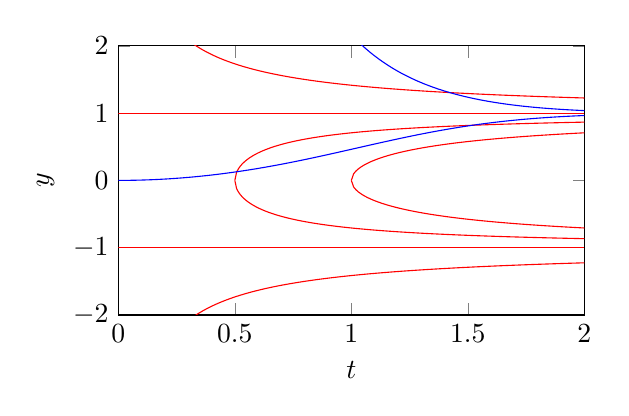
\begin{tikzpicture}
		\begin{axis}[
				%axis lines = left,
				xlabel = \(t\),
				ylabel = \(y\),
				width=7.5cm,
				height=5cm,
				xmin=0,
				xmax=2,
				ymin=-2,
				ymax=2
			]

			\addplot [
				domain=0:2,
				samples=100,
				color=red,
			]
			{1};
			%\addlegendentry{\(e^x\)}

			\addplot [
				domain=0:2,
				samples=100,
				color=red,
			]
			{-1};

			\addplot [
				domain=1:2,
				samples=100,
				color=red,
			]
			{sqrt(1-1/x)};
			\addplot [
				domain=1:2,
				samples=100,
				color=red,
			]
			{-sqrt(1-1/x)};

			\addplot [
				domain=0.5:2,
				samples=200,
				color=red,
			]
			{sqrt(1-0.5/x)};
			\addplot [
				domain=0.5:2,
				samples=200,
				color=red,
			]
			{-sqrt(1-0.5/x)};

			\addplot [
				domain=0:2,
				samples=100,
				color=red,
			]
			{sqrt(1+1/x)};
			\addplot [
				domain=0:2,
				samples=100,
				color=red,
			]
			{-sqrt(1+1/x)};

			\addplot [
				domain=0:2,
				samples=100,
				color=blue,
			]
			{(1 - e^(-x^2))/(1 + e^(-x^2))};
			\addplot [
				domain=0.1:2,
				samples=100,
				color=blue,
			]
			{(-1 - e^(-x^2))/(-1 + e^(-x^2))};
		\end{axis}
	\end{tikzpicture}
\end{wrapfigure}

Let us now draw some such isoclines on a graph, here drawn in red.
On the outermost two lines, the value of \(f\), and hence the derivative, is \(-1\).
On the lines in the centre, the value of \(f\) is \(1\) and \(0.5\), both of which are drawn so that it is easier to imagine the infinite set of isoclines.
The two horizontal lines at 1 and \(-1\) have \(f=0\).
So any solution curve that passes through these isoclines must have this gradient at the moment it intersects the line.
We can therefore visually interpolate what the gradient should be in between these known points.

Two such solution curves are drawn on this graph in blue; the one intersecting zero has \(A = 1\) in the solution for \(y\), and the one above it has \(A = -1\).
Note how, as they intersect the isoclines in red, they have exactly the gradient defined by the isocline.
Particularly, the lower solution curve intersects the same isocline twice, and therefore has this exact gradient at two distinct points --- we observe these points as the intersection points between the solution curve and the isocline.

Note also that the solutions \(y = 1\) and \(y = -1\) lie on these isoclines for all \(t\).
This is because the isoclines specify that the function has zero gradient on such a straight line, so it makes sense that the function and isocline coincide.

\subsection{Fixed points and perturbation analysis}
Points such that \(y\) is fixed for all \(t\) are called fixed points, or equilibrium points.
In our example above, \(y=1\) and \(y=-1\) are examples of fixed points.
Note that the solutions above seemed to gravitate towards \(y=1\) over time; we call such a fixed point `stable' because any slight perturbation from the value will return back to the fixed point over time.
The same is not, however, true for the \(-1\) fixed point.
It is considered `unstable' as any small perturbation will cause \(y\) to drift further and further away from \(-1\).
We can analyse this more rigorously using perturbation analysis.

Let \(y = a\) be a fixed point of \(\dot y = f(y, t)\) such that \(f(a, t) = 0\).
Then, consider some small perturbation \(\varepsilon\) from this fixed point.
Now, \(y = a + \varepsilon(t)\).
By setting the initial value of \(\varepsilon(0)\) to some arbitrarily small amount, we want to see the behaviour of \(\varepsilon(t)\) as \(t\) tends to infinity.
This way, if \(\varepsilon(t)\) goes to zero, then \(y\) will tend towards the fixed point \(a\), so the point is stable.
If \(\varepsilon(t)\) goes to any other value, then \(y\) does not tend to \(a\), so the point is unstable.

\begin{align*}
	\frac{\dd{y}}{\dd{t}} = \frac{\dd \varepsilon}{\dd{t}} & = f(a + \varepsilon, t)                                                                                                            \\
	\intertext{Expanding \(f(a + \varepsilon, t)\) as a multivariate Taylor series around \((a, t)\), we have}
	                                                       & = \underbrace{f(a, t)}_{\mathclap{=\ 0\text{ by definition}}} + \varepsilon \frac{\partial f}{\partial y}(a, t) + O(\varepsilon^2)
\end{align*}
as \(\varepsilon\) tends to zero.
So for small \(\varepsilon\), we have
\[
	\frac{\dd \varepsilon}{\dd{t}} \approx \varepsilon \frac{\partial f}{\partial y}(a, t)
\]
which is a linear ordinary differential equation for \(\varepsilon\) in terms of \(t\), as \(\frac{\partial f}{\partial y}(a, t)\) is an expression purely in terms of \(a\) and \(t\).
If (as \(t \to \infty\)) \(\varepsilon\) tends to zero then the point is stable, otherwise \(\varepsilon\) will tend to \(\pm \infty\) and the point is considered unstable.
This does not imply that \(y\) itself tends to \(\pm \infty\), just that the \(O(n^2)\) term now becomes important because \(\varepsilon\) does not tend to zero.

Note that if \(\frac{\partial f}{\partial y} = 0\), then we will need to consider the next term in the Taylor expansion, and so on, to make sure that we have an equation that lets us compute \(\varepsilon\).
In this case, however, the equation for \(\varepsilon\) will be nonlinear, as we need to consider the \(\varepsilon^2\) term, or the \(\varepsilon^3\) term, or so on.

In our example, we can deduce that \(\frac{\partial f}{\partial y} = -2yt\), so we have:
\begin{itemize}
	\item (\(y = 1\)) \begin{align*}
		      \dot \varepsilon                           & = -2(1)t \varepsilon     \\
		                                                 & = -2t\varepsilon         \\
		      \therefore \varepsilon                     & = \varepsilon_0 e^{-t^2} \\
		      \lim_{t \to \infty} \varepsilon_0 e^{-t^2} & = 0
	      \end{align*}
	      so this point is stable.
	\item (\(y = 1\)) \begin{align*}
		      \dot \varepsilon                          & = -2(-1)t \varepsilon   \\
		                                                & = 2t\varepsilon         \\
		      \therefore \varepsilon                    & = \varepsilon_0 e^{t^2} \\
		      \lim_{t \to \infty} \varepsilon_0 e^{t^2} & = \pm\infty
	      \end{align*}
	      so this point is unstable.
\end{itemize}

\subsection{Autonomous differential equations}
A special case of this is that of autonomous equations, which are defined to be differential equations of the form \(\dot y = f(y)\).
Specifically, the derivative of \(y\) does not depend on \(t\).
Therefore, near a fixed point \(y=a\), we have:
\begin{align*}
	y                         & = a + \varepsilon(t)                                   \\
	\therefore\dot\varepsilon & = \varepsilon \frac{\dd{f}}{\dd{y}}(a) = \varepsilon k
\end{align*}
where \(k\) is the constant value \(\frac{\dd{f}}{\dd{y}}(a)\).
Note that we can use normal derivatives in place of partial derivatives because \(f\) depends only on \(y\).
So the solution is
\[
	\varepsilon = \varepsilon_0 e^{kt}
\]
So, if \(k = f'(a) < 0\) then the point is stable, and if \(k = f'(a) > 0\) then the point is unstable.
This special case is useful, but it is probably only worth memorising the general case to avoid confusion, since it is simple to derive as needed.

\section{Phase portraits}
\subsection{Phase portraits}
\begin{wrapfigure}{l}{0.5\textwidth}
	\begin{tikzpicture}
		\begin{axis}[
				%axis lines = left,
				xlabel = \(c\),
				ylabel = \(\dot c\),
				width=7.5cm,
				height=5cm,
				xmin=0,
				xmax=4,
				%ymin=-1,
				%ymax=2,
				xticklabel=\empty,
				yticklabel=\empty
			]

			\addplot [
				domain=0:4,
				samples=100,
				color=red,
			]
			{(x-1)*(x-3)};

			\addplot [
				domain=0:4,
				samples=10,
				color=gray
			]
			{0};

			\addplot [
				color=blue,
				mark=*,
			]
			coordinates {
					(1,0)
				};

			\addplot [
				color=blue,
				mark=*,
			]
			coordinates {
					(3,0)
				};

			\node[above] at (axis cs:1,0) {\(a_0\)};
			\node[above] at (axis cs:3,0) {\(b_0\)};
		\end{axis}
	\end{tikzpicture}

	\begin{tikzpicture}
		\draw[-] (0,-.5) to (0,.5);
		\draw[->-=.5] (0,0) to (2,0);
		\draw[->-=.5] (5,0) to (2,0);
		\draw[->-=.5] (5,0) to (7,0);

		\filldraw[fill=black] (2,0) circle (2pt);
		\draw (5,0) circle (2pt);
		\node[above] at (2,0) {\(a_0\)};
		\node[above] at (5,0) {\(b_0\)};
	\end{tikzpicture}
\end{wrapfigure}

Another way to analyse solutions to a differential equation is using a geometrical representation of the solution, called a phase portrait.
For example,
\[
	\mathrm{NaOH} + \mathrm{HCl} \to \mathrm{H_2O} + \mathrm{NaCl}
\]
where the amount of molecules of sodium hydroxide is given by \(a(t)\), the amount of molecules of hydrochloric acid is given by \(b(t)\), the amount of molecules of water is given by \(c(t)\), and the amount of molecules of sodium chloride is given by \(d(t)\).
We can model this using the equation \(\frac{\dd{c}}{\dd{t}} = \lambda a b\).
As atoms are conserved, we have \(a = a_0 - c\) and \(b = b_0 = c\).
Then:
\[
	\frac{\dd{c}}{\dd{t}} = \lambda (a_0 - c)(b_0 - c)
\]
This is an autonomous nonlinear first order ordinary differential equation.
We can create a phase portrait by mapping out \(\frac{\dd{c}}{\dd{t}}\) as a function of \(c\), as shown in the first diagram here, which is known as a 2D phase portrait.
The second diagram, known as a 1D phase portrait, shows similar information but helps us see the behaviour of fixed points --- essentially the arrows point in the direction of motion of \(c\); if \(\dot c\) is positive then the arrows point to the right, if \(\dot c\) is negative they point to the left.
\newpage
\begin{wrapfigure}{r}{0.5\textwidth}
	\begin{tikzpicture}
		\begin{axis}[
				%axis lines = left,
				xlabel = \(y\),
				ylabel = \(\dot y\),
				width=7.5cm,
				height=5cm,
				xmin=0,
				xmax=4,
				%ymin=-1,
				%ymax=2,
				xticklabel=\empty,
				yticklabel=\empty
			]

			\addplot [
				domain=0:4,
				samples=100,
				color=red,
			]
			{-x*(x-3)};

			\addplot [
				domain=0:4,
				samples=10,
				color=gray
			]
			{0};

			\addplot [
				color=blue,
				mark=*,
			]
			coordinates {
					(0,0)
				};

			\addplot [
				color=blue,
				mark=*,
			]
			coordinates {
					(3,0)
				};

			\node[below right] at (axis cs:0,0) {\(0\)};
			\node[above] at (axis cs:3,0) {\(\lambda\)};
		\end{axis}
	\end{tikzpicture}

	\begin{tikzpicture}
		\draw[-] (0,-.5) to (0,.5);
		\draw[->-=.5] (0,0) to (5,0);
		\draw[->-=.5] (7,0) to (5,0);

		\draw (0,0) circle (2pt);
		\filldraw[fill=black] (5,0) circle (2pt);
		\node[above right] at (0,0) {\(0\)};
		\node[above] at (5,0) {\(\lambda\)};
	\end{tikzpicture}
\end{wrapfigure}

Another example is a population model.
Let \(y(t)\) denote the population.
Let \(\alpha y\) denote the birth rate, and \(\beta y\) be the death rate.
Then, we can model this using a linear model by:
\[
	\frac{\dd{y}}{\dd{t}} = \alpha y - \beta y \quad \therefore y = y_0 e^{(\alpha - \beta) t}
\]
If \(\alpha > \beta\) then we have exponential growth; if \(\alpha < \beta\) then we have exponential decay.
This is an unrealistic model, so we can use a nonlinear model to increase accuracy.
\[
	\frac{\dd{y}}{\dd{t}} = (\alpha - \beta)y - \gamma y^2
\]
When \(y\) is sufficiently large, the \(\gamma\) term becomes more relevant; here, the \(\gamma y^2\) term models the increased death rate at high populations.
Equivalently, we can write
\[
	\dot y = ry\left(1 - \frac{y}{\lambda}\right)
\]

\subsection{Fixed points in discrete equations}
Consider a first order discrete (or difference) equation of the form
\[
	x_{n+1} = f(x_n)
\]
We define the fixed points of the equation to be any value of \(x_n\) where \(x_{n+1} = x_n\) or equivalently \(f(x_n) = x_n\).
We can analyse fixed points' stability just like we can with differential equations, by using perturbation analysis.
Let \(x_f\) denote a fixed point, and then we will perturb this by a small quantity \(\varepsilon\).
\[
	f(x_f + \varepsilon) = \underbrace{f(x_f)}_{\mathclap{=x_f}} + \varepsilon \eval{\frac{\dd{f}}{\dd{x}}}_{x_f} + O(\varepsilon^2)
\]
If we let \(x_n = x_f + \varepsilon\), then
\[
	x_{n+1} \approx f(x_n) = f(x_f + \varepsilon) = x_f + \varepsilon \eval{\frac{\dd{f}}{\dd{x}}}_{x_f}
\]
\(x_f\) is stable if \(\abs{\eval{\frac{\dd{f}}{\dd{x}}}_{x_f}} < 1\), and unstable if this value is greater than 1.
This is because if the value is less than 1, \(x_{n+1}\) is closer to \(x_f\) than \(x_n\) was.

\subsection{Logistic map}
This is an extended example of analysis of discrete equations.
Let \(x_n\) be the population at generation \(n\).
Then, we use the model
\[
	\frac{x_{n+1} - x_n}{\Delta t} = \lambda x_n - \gamma x_n^2
\]
We could contrast this with a nonlinear ordinary differential equation; the left hand side of this equation is analogous to \(\frac{\dd{x}}{\dd{t}}\).
Alternatively, grouping all \(x_n\) terms on the right hand side, we have
\[
	x_{n+1} = (\lambda \Delta t + 1)x_n - \gamma \Delta t x_n^2
\]
We will actually use a slightly simplified model for this, by unifying the \(\gamma\) and \(\lambda\) terms as follows:
\[
	x_{n+1} = r x_n (1 - x_n) = f(x_n)
\]
This is known as the `logistic map'.
We will analyse the fixed points of this equation by solving \(f(x_n) = x_n\).
We have two solutions, \(x_n = 0\) and \(x_n = 1 - \frac{1}{r}\).
We can analyse their stability using perturbation analysis as before.
By letting \(f(x) = rx(1-x)\), thus removing the \(n\) index, we have
\[
	\frac{\dd{f}}{\dd{x}} = r(1-2x)
\]
At \(x_n = 0\), \(\frac{\dd{f}}{\dd{x}} = r\).
When \(0 < r < 1\), the point is stable because the next point produced by the perturbation analysis is closer to the fixed point.
If \(r > 1\) then the point is unstable.

At \(x_n = 1 - \frac{1}{r}\), \(\frac{\dd{f}}{\dd{x}} = 2 - r\).
For \(0 < r < 1\), the value of \(x_n\) is greater than 1, so it is unphysical so we discard it.
For \(r < 1 < 3\), the point is stable.
When \(r > 3\), the point is unstable.

\section{Higher order linear ODEs}
\subsection{Linear 2nd order ODEs with constant coefficients}
The general form of an equation of this type is
\[
	ay'' + by' + cy = f(x)
\]
To solve equations like this, we are going to exploit two facts: the linearity of the differential operator together with the principle of superposition.
From the definition of the derivative, we have
\[
	\frac{\dd}{\dd{x}}(y_1 + y_2) = y_1' + y_2'
\]
And similarly,
\[
	\frac{\dd^2}{\dd{x}^2}(y_1 + y_2) = y_1'' + y_2''
\]
For a linear differential operator \(D\) built from a linear combination of derivatives, for example
\[
	D = \left[ a \frac{\dd^2}{\dd{x}^2} + b\frac{\dd}{\dd{x}} + c \right]
\]
it then follows that
\[
	D(y_1 + y_2) = D(y_1) + D(y_2)
\]
We will then solve the above general equation in three steps.
\begin{enumerate}
	\item Find the complementary functions \(y_1\) and \(y_2\) which satisfy the equivalent homogeneous equation \(ay'' + by' + cy = 0\).
	\item Find a particular integral \(y_p\) which solves the original equation.
	\item If \(y_1\) and \(y_2\) are linearly independent, then \(y_1 + y_p\) and \(y_2 + y_p\) are each linearly independent solutions, which follows from the fact that \(D(y_1) = D(y_2) = 0\) and \(D(y_p) = f(x)\).
\end{enumerate}

\subsection{Eigenfunctions for 2nd order ODEs}
\(e^{\lambda x}\) is the eigenfunction of \(\frac{\dd}{\dd{x}}\), and it is also the eigenfunction of \(\frac{\dd^2}{\dd{x}^2}\), but with eigenvalue \(\lambda^2\).
More generally, it is the eigenfunction of \(\frac{\dd^n}{\dd{x}^n}\) with eigenvalue \(\lambda^n\).
In fact, \(e^{\lambda x}\) is the eigenfunction of any linear differential operator \(D\).
The equation \( ay'' + by' + cy = 0 \) can be written
\[
	\underbrace{\left[ a \frac{\dd^2}{\dd{x}^2} + b\frac{\dd}{\dd{x}} + c \right]}_{\equiv\ D} y = 0
\]
Therefore, solutions to this take the form
\[
	y_c = Ae^{\lambda x}
\]
and by substituting, we have
\[
	a \lambda^2 + b\lambda + c = 0
\]
This is known as the characteristic (or auxiliary) equation.
From the fundamental theorem of algebra, this must have two real or complex solutions.
Now, let \(\lambda_1, \lambda_2\) be these roots.

In the case that \(\lambda_1 \neq \lambda_2\), \(y_1 = Ae^{\lambda_1 x}; y_2 = Be^{\lambda_2 x}\).
In this case, the two are linearly independent and complete; they form a basis of solution space.
Therefore any other solution to this differential equation can be written as a linear combination of \(y_1\) and \(y_2\).
In general, \(y_c = Ae^{\lambda_1 x} + Be^{\lambda_2 x}\).

\subsection{Detuning}
In the case that \(\lambda_1 = \lambda_2\), this is known as a degenerate case as we have repeated eigenvalues; \(y_1\) and \(y_2\) are linearly dependent and not complete.
Let us take as an example the differential equation \(y'' - 4y' + 4y = 0\).
We try \(y_c = e^{2x}\) as \(\lambda = 2\) in this case.
We will consider a slightly modified (`detuned') equation to rectify the degeneracy.
\[
	y'' - 4y' + (4-\varepsilon^2)y = 0 \text{ where } \varepsilon \ll 1
\]
Again we will try \(y_c = e^{\lambda x}\), giving
\[
	\lambda^2 - 4 \lambda + (4 - \varepsilon^2) = 0
\]
So we have \(\lambda = 2 \pm \varepsilon\).
The complementary function therefore is \(y_c = Ae^{(2+\varepsilon)x} + Be^{(2-\varepsilon)x} = e^{2x}\left( Ae^{\varepsilon x} + Be^{-\varepsilon x} \right)\).
We will expand this in a Taylor series for small \(\varepsilon\), giving
\[
	y_c = e^{2x}\left[ (A + B) + \varepsilon x(A - B) + O(\varepsilon^2) \right]
\]
and by taking the limit, we have
\[
	\lim_{\varepsilon \to 0} y_c \approx e^{2x} \left[ (A + B) + \varepsilon x(A - B) \right]
\]
Now consider applying initial conditions to \(y_c\) at \(x = 0\).
\[
	\eval{y_c}_{x=0} = C\quad \eval{y_c'}_{x=0} = D
\]
and therefore
\[
	C = A + B;\quad D = 2C + \varepsilon(A - B)
\]
hence
\[
	A + B = O(1);\quad A - B = O\left(\frac{1}{\varepsilon}\right)
\]
in order that \(D\) is a constant.
Now, let \(\alpha = A + B; \beta = \varepsilon(A - B)\), so that we can get constants of \(O(1)\) magnitude.
Hence,
\[
	\lim_{\varepsilon \to 0} y_c = e^{2x}\left[ \alpha + \beta x \right]
\]
In general, if \(y_1(x)\) is a degenerate complementary function for linear ODEs with constant coefficients, then \(y_2 = xy_1\) is a linearly independent complementary function.

\subsection{Reduction of order}
Consider a homogeneous second-order linear ODE with non-constant coefficients.
The general form of such an equation is
\begin{equation}\label{hom_2_lin_ode_const}
	y'' + p(x) y' + q(x) y = 0
\end{equation}
Our objective is to use one solution to this equation (here denoted \(y_1\)) to find the other solution \(y_2\).
The general idea is to look for a solution of the form
\begin{equation}\label{y2_y1_reduction}
	y_2(x) = v(x)y_1(x)
\end{equation}
First, note that
\begin{align*}
	y_2'  & = v'y_1 + vy_1'             \\
	y_2'' & = v''y_1 + 2v'y_1' + vy_1''
\end{align*}
If \(y_2\) is a solution to \eqref{hom_2_lin_ode_const}, then
\[
	y_2'' + p(x) y_2' + q(x) y_2 = 0
\]
We can use \eqref{y2_y1_reduction} and collect terms, to get
\[
	v\cdot\underbrace{(y_1'' + py_1' + qy_1)}_{\mathclap{\text{0 since \(y_1\) is a solution to \eqref{hom_2_lin_ode_const}}}} + v'\cdot(2y_1' + py_1) + v''\cdot y_1 = 0
\]
Hence
\[
	v'\cdot (2y_1' + py_1) + v'' \cdot y_1 = 0
\]
This is a first order differential equation for \(v'(x)\).
Let \(u=v'\).
Then
\[
	u'y_1 + u (2y_1' + py_1) = 0
\]
This is a separable first order ODE for \(u(x)\).
So we can solve for \(u(x)\) and deduce \(v(x)\) by integration.

\subsection{Solution space}
An \(n\)th order linear ODE written
\[
	p(x)y^{(n)} + q(x) y^{(n-1)} + \cdots + r(x)y = f(x)
\]
can be used to write \(y^{(n)}(x)\) in terms of lower derivatives of \(y\).
For example, the oscillations of a mass on a spring in a damped system can be modelled as
\[
	m\ddot y = -k y - L\dot y
\]
Therefore the state of the system can be described by an \(n\)-dimensional solution vector
\begin{equation}
	\vb Y(x) \equiv \begin{pmatrix}
		y(x) \\ y'(x) \\ \vdots \\ y^{(n-1)}(x)
	\end{pmatrix}
\end{equation}
For example, an undamped oscillator modelled by \(y'' + 4y = 0\) has solutions
\[
	y_1 = \cos 2x;\quad y_2 = \sin 2x
\]
and has derivatives
\[
	y_1' = -2\sin 2x;\quad y_2' = 2\cos 2x
\]
and therefore two solution vectors are
\[
	\vb Y_1(x) = \begin{pmatrix}
		y_1 \\ y_1'
	\end{pmatrix} = \begin{pmatrix}
		\cos 2x \\ -2 \sin 2x
	\end{pmatrix}
\]
and
\[
	\vb Y_2(x) = \begin{pmatrix}
		y_2 \\ y_2'
	\end{pmatrix} = \begin{pmatrix}
		\sin 2x \\ 2 \cos 2x
	\end{pmatrix}
\]

\begin{wrapfigure}{l}{0.3\textwidth}
	\begin{tikzpicture}
		\begin{axis}[
				%axis lines = left,
				xlabel = \(y\),
				ylabel = \(\dot y\),
				width=5cm,
				height=5cm,
				xmin=-2.4,
				xmax=2.4,
				ymin=-2.4,
				ymax=2.4,
				xticklabel=\empty,
				yticklabel=\empty
			]

			\addplot [
				domain=-1:1,
				samples=200,
				color=red,
			]
			{2*sqrt(1-x^2)};
			\addplot [
				domain=-1:1,
				samples=200,
				color=red,
			]
			{-2*sqrt(1-x^2)};

			\draw[red] (axis cs: 1,0.05) -- (axis cs: 1,-0.05);
		\end{axis}
	\end{tikzpicture}
\end{wrapfigure}

We can plot the paths of these two solutions using a two-dimensional phase portrait.
In this case, both solutions follow an elliptical path.
Since \(\vb Y_1\) and \(\vb Y_2\) are linearly independent for all \(x\), any point in solution space \((y, y')\) can be written as a linear combination of these solutions.

Solutions \(y_1, y_2, \cdots, y_n\) are linearly independent for any ODE if their solution vectors \(\vb Y_1, \vb Y_2, \cdots, \vb Y_n\) are linearly independent.
A set of \(n\) linearly independent solution vectors forms a basis for the solution space of an \(n\)th order ODE.\@

\subsection{Initial conditions}
Consider initial conditions for a second order homogeneous ODE.\@
\[
	y(0) = a,\quad y'(0) = b
\]
If the general solution is
\[
	y(x) = Ay_1(x) + By_2(x)
\]
then we have the following linear system of equations
\begin{align*}
	Ay_1(0) + By_2(0)   & = a \\
	Ay_1'(0) + By_2'(0) & = b
\end{align*}
which is a system of two equations for two unknowns.
Or alternatively,
\[
	\underbrace{\begin{pmatrix}
			y_1(0)  & y_2(0)  \\
			y_1'(0) & y_2'(0)
		\end{pmatrix}}_{\equiv M}
	\begin{pmatrix}
		A \\ B
	\end{pmatrix}
	=
	\begin{pmatrix}
		a \\b
	\end{pmatrix}
\]
Unique solutions for \(A\) and \(B\) exist if \(\det M \neq 0\).

\subsection{The fundamental matrix and the Wro\'nskian}
The fundamental matrix is a matrix formed by placing solution vector \(\vb Y_i\) in the \(i\)th column.
The Wro\'nskian, denoted \(W(x)\), is the determinant of the fundamental matrix.
\[
	W(x) \equiv \begin{vmatrix}
		\vdots  & \vdots  &        & \vdots  \\
		\vb Y_1 & \vb Y_2 & \cdots & \vb Y_n \\
		\vdots  & \vdots  &        & \vdots
	\end{vmatrix} = \begin{vmatrix}
		y_1         & y_2         & \cdots & y_n         \\
		y_1'        & y_2'        & \cdots & y_n'        \\
		\vdots      & \vdots      & \ddots & \vdots      \\
		y_1^{(n-1)} & y_2^{(n-1)} & \cdots & y_n^{(n-1)}
	\end{vmatrix}
\]
For a second order ODE:\@
\begin{equation}\label{wronskian2}
	W(x) = \begin{vmatrix}
		y_1 & y_2 \\ y_1' & y_2'
	\end{vmatrix}
	= y_1y_2' - y_2y_1'
\end{equation}
The solution vectors are linearly independent if \(W(x) \neq 0\).
This is a convenient test for the linear independence of two solution vectors.
In our example above, we had
\[
	W(x) = \begin{vmatrix}
		\cos 2x   & \sin 2x  \\
		-2\sin 2x & 2\cos 2x
	\end{vmatrix}
	= 2\cos^2 2x + 2\sin^2 2x = 2 \neq 0
\]
So the solution vectors are linearly independent for all \(x\).

\subsection{Using the Wro\'nskian to find the original ODE}
If \(\vb Y_1\) and \(\vb Y_2\) are linearly dependent, then \(W(x) = 0\).
Suppose that a third solution \(y(x)\) is a linear combination of \(y_1(x)\) and \(y_2(x)\).
Then the solution vectors \(\vb Y, \vb Y_1, \vb Y_2\) are a linearly dependent set.
Hence
\[
	\begin{vmatrix}
		y   & y_1   & y_2   \\
		y'  & y_1'  & y_2'  \\
		y'' & y_1'' & y_2''
	\end{vmatrix}
	= 0
\]
For \(y_1 = \cos 2x\) and \(y_2 = \sin 2x\), we can deduce the original differential equation that produced these solutions by solving for \(y\).
\begin{align*}
	\begin{vmatrix}
		y   & \cos 2x   & \sin 2x    \\
		y'  & -2\sin 2x & 2 \cos 2x  \\
		y'' & -4\cos 2x & -4 \sin 2x
	\end{vmatrix}
	                                             & = 0 \\
	\implies y(8\sin^2 2x + 8\cos^2 2x)          &     \\
	- y'(-4 \cos 2x \sin 2x + 4 \cos 2x \sin 2x) &     \\
	+ y''(2\cos^2 2x + 2\sin^2 2x)               & = 0 \\
	\implies y'' + 4y                            & = 0
\end{align*}
Note that if \(W(x) = 0\), this does not necessarily imply linear dependence.

\subsection{Abel's theorem}
Consider a second order homogeneous ODE:\@
\[
	y'' + p(x)y' + q(x)y = 0
\]
\begin{theorem}[Abel's Theorem]
	If \(p(x)\) and \(q(x)\) are continuous on an interval \(I\), then the Wro\'nskian \(W(x)\) is either zero or nonzero for all \(x \in I\).
\end{theorem}
\begin{proof}
	Let \(y_1, y_2\) be solutions to the equation.
	Then
	\begin{align}
		\label{abelproof1} y_2(y_1'' + p(x)y_1' + q(x)y_1) & = 0 \\
		\label{abelproof2} y_1(y_2'' + p(x)y_2' + q(x)y_2) & = 0
	\end{align}
	Now, calculating \eqref{abelproof2} \(-\) \eqref{abelproof1}, we get
	\begin{equation}\label{abelproof3}
		(y_1y_2'' - y_2y_1'') + p(x)(y_1y_2' - y_2y_1') = 0
	\end{equation}
	As we are solving a second order equation, \(W(x) = y_1y_2' - y_2y_1'\) and therefore
	\[
		\frac{\dd{W}}{\dd{x}} = y_1y_2'' + y_1'y_2' - y_2'y_1' - y_2y_1'' = y_1y_2'' - y_2y_1''
	\]
	Note that these are the coefficients in \eqref{abelproof3}.
	We have therefore
	\begin{equation}\label{abelproof4}
		W' + pW = 0
	\end{equation}
	Then by separating variables:
	\begin{align*}
		\frac{\dd{W}}{W}              & = -p(x)\dd{x}                         \\
		\int_{x_0}^x \frac{\dd{W}}{W} & = -\int_{x_0}^x p(u)\dd{u}            \\
		W(x)                          & = W(x_0)e^{-\int_{x_0}^x p(u) \dd{u}}
	\end{align*}
	This last equation is known as Abel's Identity, and is very important.
	Since \(p(x)\) is continuous on \(I\) with \(x \in I\), it is bounded and therefore integrable.
	Therefore \(e^{-\int_{x_0}^x p(u) \dd{u}} \neq 0\).
	It follows that if \(W(x_0) = 0\) then \(W(x) = 0\) for all \(x\).
	Likewise, if \(W(x_0) \neq 0\), then \(W(x) \neq 0\) for all \(x\) (on the interval).
\end{proof}
\begin{corollary}
	If \(p(x) = 0\), then \(W = W_0\) which is a constant.
\end{corollary}
Note that we can use this to find \(W(x)\) without actually solving the differential equation itself.
For example, Bessel's Equation
\[
	x^2y'' + xy' + (x^2 - n^2)y = 0
\]
has no closed form solutions, but the Wro\'nskian can be calculated be rewriting it as
\[
	y'' + \frac{1}{x}y' + \frac{x^2-n^2}{x^2}y = 0
\]
and by Abel's Identity,
\begin{align*}
	W(x) & = W_0 e^{-\int_{x_0}^x \frac{1}{u} \dd{u}} \\
	     & = W_0 e^{-\ln x}                           \\
	     & = \frac{W_0}{x}
\end{align*}

\subsection{Using Abel's identity}
We can find a second solution \(y_2\) given a solution \(y_1\) using a reduction of order method, but we can also use Abel's Identity.
\[
	y_1y_2' - y_2y_1' = W_0 e^{-\int_{x_0}^x p(u) \dd{u}}
\]
This is a first order ODE for \(y_2\) which we can now solve:
\[
	\frac{y_1y_2' - y_2y_1'}{y_1^2} =  \frac{W_0}{y_1^2} e^{-\int_{x_0}^x p(u) \dd{u}}
\]
The left hand side is exactly the quotient rule, giving
\[
	\dv{x}\frac{y_2}{y_1} = \frac{W_0}{y_1^2} e^{-\int_{x_0}^x p(u) \dd{u}}
\]
which can be solved to give \(y_2\) as a function of \(y_1\) and \(W\).

\subsection{Abel's theorem in higher dimensions}
Any linear \(n\)th order ODE can be written
\[
	\vb Y' + A(x) \vb Y = 0
\]
where \(A\) is a matrix; this converts an \(n\)th order ODE into a system of \(n\) first order ODEs.
This will be discussed later in the course.
It can be shown that this generalisation of Abel's Identity
\[
	W' + \tr(A)W = 0
\]
holds, and hence
\[
	W' = W_0e^{-\int_{x_0}^x \tr(A) \dd{u}}
\]
and Abel's theorem holds.
This is shown on example sheet 3, Question 7.

\subsection{Equidimensional equations}
An ODE is equidimensional if the differential operator is unaffected by a multiplicative scaling.
For example, rescaling
\[
	x \mapsto X = \alpha x
\]
where \(\alpha \in \mathbb R\).
The general form for a second order equidimensional equation is
\begin{equation}\label{equidimensional1}
	ax^2 y'' + bxy' + cy = f(x)
\end{equation}
where \(a, b, c\) are constant.
Note, \(\frac{\dd}{\dd{X}} = \frac{1}{\alpha}\frac{\dd}{\dd{x}}\), and \(\frac{\dd^2}{\dd{X}^2} = \frac{1}{\alpha^2}\frac{\dd}{\dd{x}^2}\), so plugging this into \eqref{equidimensional1} gives
\[
	aX^2\frac{\dd^2 y}{\dd{X}^2} + bX\frac{\dd{y}}{\dd{X}} + cy = f\left(\frac{X}{\alpha}\right)
\]
The left hand side was unaffected by this rescaling, so the equation is equidimensional.

There are two main methods for solving equidimensional equations.
\begin{enumerate}
	\item Note that \(y = x^k\) is an eigenfunction of the differential operator \(x\frac{\dd}{\dd{x}}\).
	      Inspired by this, to solve \eqref{equidimensional1} we will look for solutions of the form \(y=x^k\), so we have
	      \[
		      ak(k-1) + bk + c = 0
	      \]
	      We can simply solve this quadratic for two roots \(k_1\) and \(k_2\).
	      If \(k_1 \neq k_2\), then the complementary function is
	      \[
		      y_c = Ax^{k_1} + Bx^{k_2}
	      \]
	\item If \(k_1 = k_2\), then the substitution \(z = \ln x\) turns \eqref{equidimensional1} into an equation with constant coefficients.
	      \[
		      a \frac{\dd^2 y}{\dd{z}^2} + (b-a)\frac{\dd{y}}{\dd{z}} + cy = f(e^z)
	      \]
	      (TODO verify this).
	      Because this has constant coefficients, our complementary functions will be of the form \(y = e^{\lambda z}\), which can be solved as usual.
	      \[
		      y_c = Ae^{\lambda_1 z} + Be^{\lambda_2 z} = Ax^{\lambda_1} + Bx^{\lambda_2}
	      \]
	      which is the same form as above.
	      In this form, it is easier to see that if the two solutions \(\lambda_1\), \(\lambda_2\) are the same, then
	      \[
		      y_c = Ae^{\lambda_1 z} + Bze^{\lambda_1 z} = Ax^{k_1} + Bx^{k_1}\ln x
	      \]
\end{enumerate}

\section{Forced second order ODEs}
We want to find methods for finding the particular integral of forced second order ODEs.
\subsection{Guesswork}
Here, \(f(x)\) is the forcing term.

\begin{tabular}{c c}
	Form of \(f(x)\)                        & Form of \(y_p(x)\)                          \\\midrule
	\(e^{mx}\)                              & \(Ae^{mx}\)                                 \\
	\(\sin(kx)\) or \(\cos(kx)\)            & \(A\sin(kx) + B\cos(kx)\)                   \\
	\(x^n\) or an \(n\)th degree polynomial & \(a_n x^n + a_{n-1}x^{n-1} + \cdots + a_0\)
\end{tabular}

In general:
\begin{enumerate}
	\item Insert our guess into the equation;
	\item Equate coefficients of functions;
	\item Solve for unknown coefficients.
\end{enumerate}

\subsection{Variation of parameters}
This is a method for finding the particular integral \(y_p\) given complementary functions \(y_1\), \(y_2\), which are assumed to be linearly independent, with solution vectors
\[
	\vb Y_1 = \begin{pmatrix}
		y_1 \\ y_1'
	\end{pmatrix};\quad \vb Y_2 = \begin{pmatrix}
		y_2 \\ y_2'
	\end{pmatrix}
\]
Suppose that the solution vector for \(y_p\) satisfies
\begin{equation}\label{varparam1}
	\vb Y_p = \begin{pmatrix}
		y_p \\ y_p'
	\end{pmatrix} = u(x)\vb Y_1 + v(x)\vb Y_2
\end{equation}
This is not a linear combination of \(\vb Y_1\) and \(\vb Y_2\), but we can treat it as a linear combination at a fixed \(x\) point (just as a way to visualise it).
We want to find equations for \(u(x)\) and \(v(x)\).
By comparing components of the vectors on the left and right, we have
\begin{align*}
	y_p  & = uy_1 + vy_2 \tag{a}   \\
	y_p' & = uy_1' + vy_2' \tag{b} \\
\end{align*}
So therefore,
\[
	\frac{\dd}{\dd{x}}(\mathrm a) \implies y_p' = u'y_1 + uy_1' + v'y_2 + vy_2' \tag{c}
\]
\[
	(\mathrm c) - (\mathrm b) \implies u'y_1 + v'y_2 = 0 \tag{d}
\]
Now:
\[
	\frac{\dd}{\dd{x}}(\mathrm b) \implies y_p'' = uy_1'' + u'y_1' + v'y_2' + vy_2'' \tag{e}
\]
If \(y_p'' + p(x)y_p' + q(x)y_p = f(x)\), then
\[
	(\mathrm e) + p(\mathrm b) + q(\mathrm a) = f(x)
\]
But also, \(y_1\) and \(y_2\) satisfy the differential equation
\[
	y_c'' + py_c' + qy_c = 0\quad y_c \in \{ y_1, y_2 \}
\]
After we substitute in and cancel a lot of terms, we have
\[
	u'y_1' + v'y_2' = f(x) \tag{f}
\]
Combining (d) and (f), we can deduce \(u\) and \(v\).
\[
	\underbrace{\begin{pmatrix}
			y_1 & y_2 \\ y_1' & y_2'
		\end{pmatrix}}_{\mathclap{\text{fundamental matrix}}} \begin{pmatrix}
		u' \\ v'
	\end{pmatrix} = \begin{pmatrix}
		0 \\ f
	\end{pmatrix}
\]
So as long as \(y_1\) and \(y_2\) are linearly independent, i.e.\ the Wro\'nskian is nonzero, we can write an equation for \(u'\) and \(v'\).
\[
	\begin{pmatrix}
		u' \\ v'
	\end{pmatrix} = \frac{1}{W(x)}\begin{pmatrix}
		y_2' & -y_2 \\ y_1' & y_1
	\end{pmatrix} \begin{pmatrix}
		0 \\ f
	\end{pmatrix}
\]
or explicitly,
\begin{align*}
	u' & = \frac{-y_2 f}{W} \\
	v' & = \frac{y_1 f}{W}
\end{align*}
and therefore
\[
	y_p = y_2 \int^x \frac{y_1(t) f(t)}{W(t)}\dd{t} - y_1 \int^x \frac{y_2(t) f(t)}{W(t)}\dd{t}
\]

\subsection{Forced oscillating systems: transients and damping}
Many physical systems have a restoring force and damping (e.g.
friction).
For example, the suspension of a car could be modelled with \(y(t)\), where \(y\) is the height of the wheel, given by
\[
	M\ddot y = F(t) - \underbrace{ky}_{\text{spring}} - \underbrace{L\dot y}_{\text{damper}}
\]
In standard form, we have
\[
	\ddot y + \frac{L}{M} \dot y + \frac{k}{M} y = \frac{F(t)}{M}
\]
Let \(\tau = \sqrt{\frac{k}{M}} t\).
Then we can rewrite this equation using a single parameter:
\[
	y'' + 2Ky' + y = f(\tau)
\]
where \(y' = \frac{\dd{y}}{\dd \tau}\), \(K = \frac{L}{2\sqrt{kM}}\), \(f = \frac{F}{k}\).
Our unforced system is described here by one parameter \(K\).

In the case of the unforced response (also known as the free or natural response), we have \(f=0\), so
\[
	y'' + 2Ky' + y = 0
\]
Solving by the characteristic equation, we see
\[
	\lambda = -K \pm \sqrt{K^2 - 1}
\]
There are a number of cases here.
\begin{enumerate}
	\item (\(K < 1\)) This produces a decaying oscillation, known as `underdamped'.
	      \(\lambda_1, \lambda_2\) are both complex, and therefore
	      \[
		      y = e^{-K\tau}\left[A\sin(\sqrt{1-K^2}\tau) + B\cos(\sqrt{1-K^2}\tau)\right]
	      \]
	      The period is \(\frac{2\pi}{\sqrt{1-K^2}}\).
	      As \(K\) tends to 1, the period tends to \(\infty\).
	\item (\(K = 1\)) This is the degenerate case, \(\lambda_1 = \lambda_2 = -K\).
	      We can use detuning to deduce
	      \[
		      y = e^{-K\tau} (A + B\tau)
	      \]
	\item (\(K > 1\)) Here, we have two negative real roots \(\lambda_1, \lambda_2\); this situation is known as `overdamped'.
	      \[
		      y = Ae^{\lambda_1 \tau} + Be^{\lambda_2 \tau}
	      \]
\end{enumerate}
Note that the unforced response decays in all cases.

\subsection{Sinusoidal forcing}
Let
\[
	\ddot y + \mu \dot y + \omega_0^2 y = \sin \omega t
\]
Now let us guess \(y_p = A\sin \omega t + B\cos \omega t\).
Equating coefficients of \(\sin\omega t\) gives
\[
	-A\omega^2 - B\mu\omega + \omega_0^2A = 1 \tag{a}
\]
and equating \(\cos\omega t\) gives
\[
	-B\omega^2 + A\mu\omega + \omega_0^2B = 0 \tag{b}
\]
Then:
\[
	(\text b) \implies A = B \frac{\omega^2 - \omega_0^2}{\mu\omega}
\]
\[
	(\text a) \implies A(\omega_0^2 - \omega^2) = 1 + B\mu\omega
\]
So
\[
	A = \frac{\omega_0^2 - \omega^2}{(\omega_0^2 - \omega^2)^2 + \mu^2\omega^2}
\]
\[
	B = \frac{-\mu\omega}{(\omega_0^2 - \omega^2)^2 + \mu^2\omega^2}
\]
Altogether, we have
\[
	y_p = \frac{1}{(\omega_0^2 - \omega^2)^2 + \mu^2\omega^2}\left[ (\omega_0^2 - \omega^2)\sin\omega t - \mu \omega \cos \omega t \right]
\]
Drawing an example of this kind of particular integral in red (with the complementary function in blue), we can see the following:

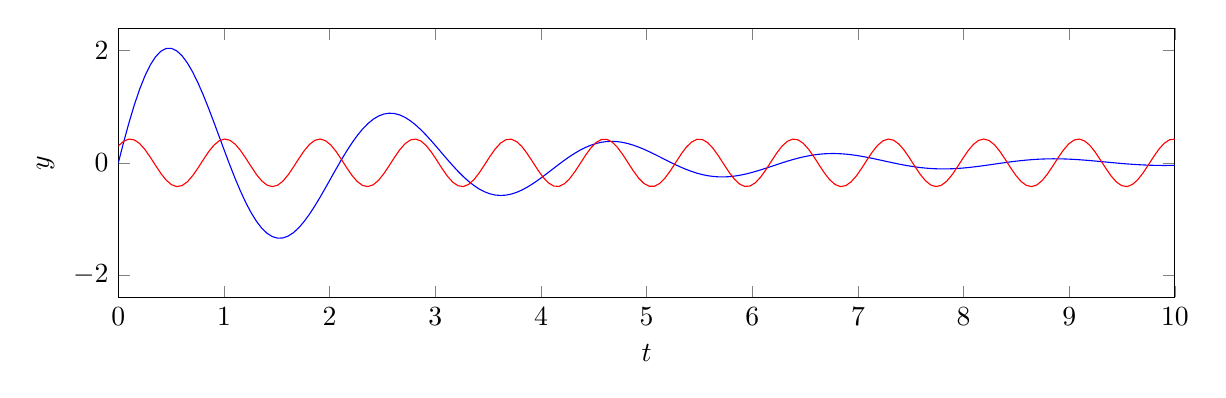
\begin{tikzpicture}
	\begin{axis}[
			%axis lines = left,
			xlabel = \(t\),
			ylabel = \(y\),% \(y = y_c + y_p\),
			width=15cm,
			height=5cm,
			xmin=0,
			xmax=10,
			ymin=-2.4,
			ymax=2.4
			%xticklabel=\empty,
			%yticklabel=\empty
		]

		\addplot [
			domain=0:10,
			samples=200,
			color=blue
		]
		{2.5*e^(-0.4*x)*sin(3*deg(x))};

		\addplot [
			domain=0:10,
			samples=200,
			color=red
		]
		{0.3*(sin(7*deg(x)) + cos(7*deg(x)))};
	\end{axis}
\end{tikzpicture}

And adding both together to form a particular solution gives:

\begin{tikzpicture}
	\begin{axis}[
			%axis lines = left,
			xlabel = \(t\),
			ylabel = \(y\),% \(y = y_c + y_p\),
			width=15cm,
			height=5cm,
			xmin=0,
			xmax=10,
			ymin=-2.4,
			ymax=2.4
			%xticklabel=\empty,
			%yticklabel=\empty
		]

		\addplot [
			domain=0:10,
			samples=200,
			color=black
		]
		{2.5*e^(-0.4*x)*sin(3*deg(x)) + 0.3*(sin(7*deg(x)) + cos(7*deg(x)))};
	\end{axis}
\end{tikzpicture}

Let us make a few comments about these forced oscillations.
\begin{itemize}
	\item The complementary function gives us the transient (short-term) response to the initial conditions.
	\item The particular integral gives the long-term response to the forcing term.
	\item In some sense, the system `forgets' about the initial conditions over time due to the damping term.
\end{itemize}

\subsection{Resonance in undamped systems}
What happens if \(\omega = \omega_0\)?
If \(\mu \neq 0\) (i.e.\ it is a damped system), then
\[
	\lim_{\omega \to \omega_0} y_p = \frac{-\cos\omega_0 t}{\mu\omega_0}
\]
This is a finite amplitude oscillation.
Note that the amplitude increases with decreasing \(\mu\), so clearly this solution has a problem at \(\mu = 0\).
To work with this, we'll let
\[
	\ddot y + \omega_0^2 y = \sin\omega_0 t
\]
We will use detuning to get solutions for this equation.
Consider instead
\[
	\ddot y + \omega_0^2 y = \sin\omega t
\]
where \(\omega \neq \omega_0\).
We will guess that the particular integral is of the form \(y_p = C\sin\omega t\) since by inspection there cannot be any cosine terms.
\[
	C(-\omega^2 + \omega_0^2) = 1
\]
\[
	\therefore y_p = \frac{1}{\omega_0^2 - \omega^2}\sin\omega t
\]
As the system is linear in \(y\) and its derivatives, we can freely add some multiple of the complementary function and it will remain a solution.
\[
	y_p = \frac{1}{\omega_0^2 - \omega^2}\sin\omega t + A \sin\omega_0 t
\]
Now let us pick \(A = \frac{-1}{\omega_0^2 - \omega^2}\), so
\[
	y_p = \frac{\sin \omega t - \sin \omega_0 t}{\omega_0^2 - \omega^2}
\]
Rewriting this using angle addition and subtraction identities:
\[
	y_p = \frac{2}{\omega_0^2 - \omega^2}\left[ \cos\left( \frac{\omega + \omega_0}{2}t \right) \sin\left( \frac{\omega - \omega_0}{2}t \right) \right]
\]
For convenience, let \(\Delta\omega \equiv \omega_0 - \omega\), and therefore \(\frac{\omega + \omega_0}{2} = w_0 - \frac{1}{2}\Delta\omega\).
\[
	y_p = \frac{-2}{\Delta\omega(\omega_0 + \omega)}\left[ \cos\left( \left(\omega_0 - \frac{\Delta\omega}{2}\right)t \right) \sin\frac{\Delta\omega t}{2} \right]
\]
In the following diagram, \(y_p\) is drawn in blue, with the sine term (in red) acting as an envelope for the higher-frequency cosine term.
The phenomenon visible here is known as `beating', as an oscillator with a fundamental frequency slightly different to the forcing frequency will begin oscillating then stop, and repeat this cycle.

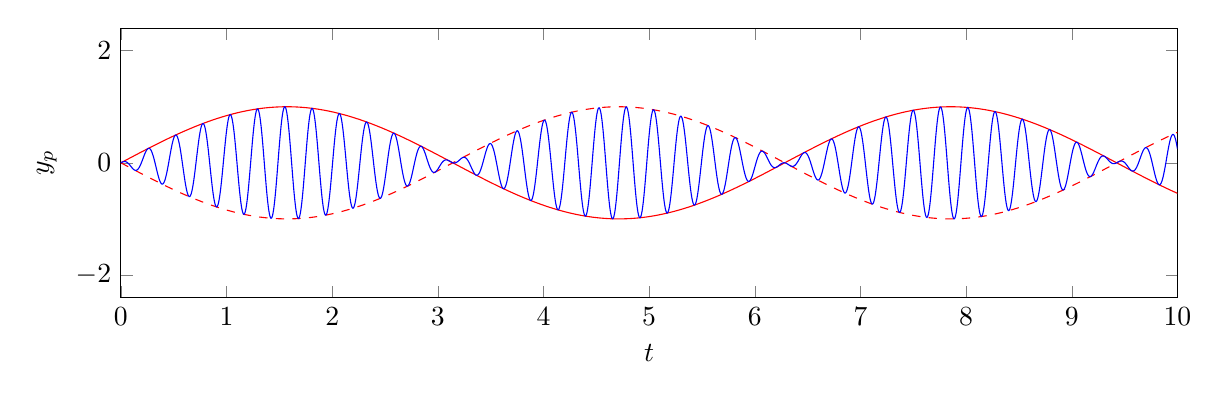
\begin{tikzpicture}
	\begin{axis}[
			%axis lines = left,
			xlabel = \(t\),
			ylabel = \(y_p\),% \(y = y_c + y_p\),
			width=15cm,
			height=5cm,
			xmin=0,
			xmax=10,
			ymin=-2.4,
			ymax=2.4
			%xticklabel=\empty,
			%yticklabel=\empty
		]

		\addplot [
			domain=0:10,
			samples=200,
			color=red
		]
		{sin(deg(x))};
		\addplot [
			dashed,
			domain=0:10,
			samples=200,
			color=red
		]
		{-sin(deg(x))};

		\addplot [
			domain=0:10,
			samples=2000,
			color=blue
		]
		{cos(24.3*deg(x))*sin(deg(x))};
	\end{axis}
\end{tikzpicture}

As we reduce \(\Delta\omega\) to zero, we have
\[
	\lim_{\Delta\omega\to 0} \sin\left(\frac{\Delta\omega}{2}t\right) \approx \frac{\Delta\omega}{2}t
\]
So
\begin{align*}
	\lim_{\Delta\omega\to 0}
	 & \approx \frac{-2}{\Delta\omega(\omega_0 + \omega_0)} \cos(\omega_0t)\left(\frac{\Delta\omega}{2}t\right) \\
	 & \approx \frac{-2t}{\omega_0} \cos\omega_0t                                                               \\
\end{align*}
This is linear growth in amplitude over time.
This increase is unbounded an in undamped system.
Note that \(y_p\) takes the form of one of the complementary functions multiplied by the independent variable.

\subsection{Impulses and point forces}
Consider a system that experiences a sudden force, for example a car's suspension when driving over a speed bump.
Let us define \(y\) to be the displacement from the undisturbed height of the suspension.
Let the car's mass be \(M\).
In a small finite window \(\varepsilon\) around some time \(T\), the excess force \(F\) (the forcing term) on the system is greater than zero.
As \(\varepsilon\) tends to zero, the force becomes a sudden impulse.
Let us model this using the equation
\[
	M\ddot y = F(t) - ky - L\dot y
\]
We can see that before time \(T\), \(y=0\).
After this point, there is some kind of oscillation.
Note that the value of \(y\) is always continuous (otherwise this would violate many laws of physics), but the derivative is not necessarily continuous at the point \(T\).
Let us integrate the equation above in time from \(T - \varepsilon\) to \(T + \varepsilon\).
\begin{equation}\label{impulse1}
	\lim_{\varepsilon \to 0} \left[ M[\dot y]_{T - \varepsilon}^{T + \varepsilon} = \int_{T - \varepsilon}^{T + \varepsilon} F(t) \dd{t} - k \underbrace{\int_{T - \varepsilon}^{T + \varepsilon} y \dd{t}}_{0\text{ if \(y\) is finite}} - L\underbrace{[y]_{T - \varepsilon}^{T + \varepsilon}}_{0\text{ if \(y\) is continuous}} \right]
\end{equation}
We now can define the impulse \(I\) to be
\[
	I = \lim_{\varepsilon \to 0} \int_{T - \varepsilon}^{T + \varepsilon} F(t) \dd{t}
\]
Hence
\[
	\eqref{impulse1} \implies I = \lim_{\varepsilon \to 0} M[\dot y]_{T - \varepsilon}^{T + \varepsilon}
\]
So if the impulse is nonzero, the velocity \(\dot y\) experiences a sudden change, so it is discontinuous at \(T\).
The value of this sudden change in velocity depends on the integral of the force.

\section{Impulse forcing}
\subsection{Dirac delta function}
First let us consider a family of functions \(D(t; \varepsilon)\) defined by
\[
	\lim_{\varepsilon \to 0} D(t; \varepsilon) = 0;\quad\forall t \neq 0
\]
\[
	\int_{-\infty}^\infty D(t;\varepsilon) \dd{t} = 1
\]
For example,
\[
	D(t; \varepsilon) = \frac{1}{\varepsilon\sqrt{\pi}}e^{\frac{-t^2}{\varepsilon^2}}
\]
We can now define the Dirac delta function \(\delta(t) = \lim_{\varepsilon \to 0} D(t; \varepsilon)\).
It has a number of interesting properties:
\begin{itemize}
	\item \(\delta(x) = 0\) for all nonzero \(x\)
	\item \(\int_{-\infty}^\infty \delta(t) \dd{t} = 1\)
	\item (sampling property) For a continuous function \(g(x)\):
	      \[
		      \int_{-\infty}^\infty g(x)\delta(x) \dd{x} = g(0)\int_{-\infty}^\infty \delta(x) \dd{x} = g(0)
	      \]
	      And more generally,
	      \[
		      \int_a^b g(x)\delta(x-x_0) \dd{x} = \begin{cases}
			      g(x_0) & a \leq x_0 \leq b \\
			      0      & \text{otherwise}
		      \end{cases}
	      \]
\end{itemize}

\subsection{Heaviside step function}
Exploiting the definition of the \(\delta\) function, we will define the Heaviside step function \(H(x)\) by
\[
	H(x) \equiv \int_{-\infty}^x \delta(t) \dd{t}
\]
Here are some of its properties:
\begin{itemize}
	\item \(H(x) = 0\) for \(x < 0\)
	\item \(H(x) = 1\) for \(x > 0\)
	\item \(H(0)\) is undefined
\end{itemize}

\subsection{Ramp function}
We define the ramp function \(r(x)\) by
\[
	r(x) \equiv \int_{-\infty}^x H(t) \dd{t}
\]
This function is shaped like a ramp:
\[
	r(x) = \begin{cases}
		0 & x < 0    \\
		x & x \geq 0
	\end{cases}
\]
These functions get `smoother' the more times we integrate.

\subsection{Delta function forcing}
Consider a linear second order ODE of the form
\begin{equation}\label{dirac2ode}
	y'' + p(x)y' + q(x)y = \delta(x)
\end{equation}
The key principle is that the highest order deriative `inherits' the level of discontinuity from the forcing term, since if any other derivative were to contain the discontinuous function, then the next higher derivative would only be more discontinuous.
So, \(y''\) behaves somewhat like \(\delta\).
Here, we will denote this \(y'' \sim \delta\) --- this is extremely non-standard notation, however.

Now, since \(\delta(x) = 0\) for all nonzero \(x\), then
\[
	y''+py'+qy=0 \text{ for } x<0, x>0
\]
We will essentially have two solutions for \(y\); one for before the impulse and one after.
We need to combine these together somehow to create the resultant \(y\) solution.
But this leaves four constants of integration, so surely we can't solve it.
Luckily, \(y\) satisfies certain `jump conditions' (the analogous concept to initial conditions in this context):
\begin{itemize}
	\item \(y(x)\) is continuous at \(x=0\) because \(y'' \sim \delta \implies y' \sim H \implies y \sim r\).
	      More precisely:
	      \[
		      \lim_{\varepsilon \to 0} [y]_{x=-\varepsilon}^{x=\varepsilon} = 0
	      \]
	\item \(y'(x)\) is has a jump of 1 at \(x=0\) because \(y'' \sim \delta \implies y' \sim H\).
	      Again we can formulate this intuition more precisely by integrating \eqref{dirac2ode} around a small window \(\varepsilon\):
	      \begin{align*}
		      \lim_{\varepsilon \to 0} \int_{-\varepsilon}^\varepsilon y'' + p(x)y' + q(x)y \dd{x} & = \lim_{\varepsilon \to 0} \int_{-\varepsilon}^\varepsilon \delta(x) \dd{x} \\
		      \lim_{\varepsilon \to 0} [y']_{x=-\varepsilon}^{x=\varepsilon}                       & = 1
	      \end{align*}
\end{itemize}
As a more concrete example, let us solve
\[
	y'' - y = 3 \delta\left(x - \frac{\pi}{2}\right)
\]
where
\[
	x = 0, x = \pi \implies y = 0
\]
First, let us solve the interval \(0 \leq x < \frac{\pi}{2}\).
\begin{align*}
	y'' - y                              & = 0                                              \\
	y                                    & = Ae^x + Be^{-x}                                 \\
	\text{or } y                         & = A \sinh x + B \cosh x \text{ redefining } A, B \\
	(y = 0 \text{ at } x = 0) \implies y & = A \sinh x
\end{align*}
Similarly, between \(\frac{\pi}{2} < x \leq \pi\) (since the equation is invariant under the transformation \(x \mapsto \pi - x\)):
\[
	y = C \sinh (\pi - x)
\]
Now, we can apply two jump conditions to solve for these constants:
\begin{itemize}
	\item Integrating the differential equation over a small region:
	      \[
		      \lim_{\varepsilon \to 0} [y]_{x = \frac{\pi}{2} - \varepsilon}^{x = \frac{\pi}{2} + \varepsilon} = 3
	      \]
	      Hence, taking the derivatives of our two solutions:
	      \[
		      -A\cosh\frac{\pi}{2} - C\cosh\frac{\pi}{2} = 3
	      \]
	\item Since the \(y\) term is continuous:
	      \[
		      [y]_{x = \frac{\pi}{2} - \varepsilon}^{x = \frac{\pi}{2}} = 0
	      \]
	      \[
		      A \sinh \frac{\pi}{2} = C \sinh \frac{\pi}{2} \implies A = C
	      \]
\end{itemize}
Using both jump conditions, we have \(A = C = \frac{-3}{2\cosh \frac{\pi}{2}}\).
So our general solution is
\[
	y = \begin{cases}
		\frac{-3\sinh x}{2\cosh \frac{\pi}{2}}         & 0 \leq x < \frac{\pi}{2}   \\
		\frac{-3\sinh (\pi - x)}{2\cosh \frac{\pi}{2}} & \frac{\pi}{2} < x \leq \pi
	\end{cases}
\]
Note that often when working with limits as \(\varepsilon \to 0\), we simply elide the limit sign since it is so ubiquitous.

\subsection{Heaviside function forcing}
Consider
\begin{equation}\label{heaviside0}
	y'' + p(x)y' + q(x)y = H(x - x_0)
\end{equation}
Now, \(y(x)\) satisfies
\begin{align}
	y'' + py' + qy & = 0\quad (x<x_0) \label{heaviside1} \\
	y'' + py' + qy & = 1\quad (x>x_0) \label{heaviside2}
\end{align}
Evaluating \eqref{heaviside0} on either side of \(x_0\), we have
\[
	[y'']_{x_0^-}^{x_0^+} + p(x_0)[y']_{x_0^-}^{x_0^+} + q(x_0)_{x_0^-}^{x_0^+} = 1
\]
If \(y'' \sim H\) then \(y' \sim r\) and then \(y \sim \int r\).
Hence, \(y'\) and \(y\) are both continuous.
So our jump conditions are
\begin{itemize}
	\item \([y']_{x_0^-}^{x_0^+} = 0\)
	\item \([y]_{x_0^-}^{x_0^+} = 0\)
\end{itemize}
We can use the two initial or boundary conditions, along with the two jump conditions, to find the four constants in the solutions to \eqref{heaviside1} and \eqref{heaviside2}.

\section{Discrete equations and the method of Frobenius}
\subsection{Higher order discrete equations}
The general form of an \(m\)th order linear discrete equation with constant coefficients is
\begin{equation}\label{mlindiscrete}
	a_m y_{n+m} + a_{m-1}y_{n+m-1} + \dots + a_1y_{n+1} + a_0y_n = f_n
\end{equation}
To solve such an equation, we will exploit some principles used to solve higher order differential equations.

To apply eigenfunction properties, we will define a difference operator \(D[y_n] = y_{n+1}\).
Then, \(D\) has eigenfunction \(y_n = k^n\) for \(k\) constant, since \(D[k^n] = k^{n+1} = k \cdot k^n = ky_n\).

To apply linearity, notice that \eqref{mlindiscrete} is linear in \(y\), so the general solution \(y_n = y_n^{(c)} + y_n^{(p)}\) where \(y^{(c)}\) is the complementary function and \(y^{(p)}\) is the particular integral.

As an example, let us consider a second order difference equation
\[
	a_2 y_{n+2} + a_1 y_{n+1} + a_0 y_n = f_n
\]
We will first try to solve the homogeneous equation, letting \(f=0\).
\[
	a_2 y_{n+2} + a_1 y_{n+1} + a_0 y_n = 0
\]
We will look for solutions of the form of the eigenfunction: \(y_n = k^n\).
\[
	a_2 k^2 + a_1 k + a_0 = 0
\]
This quadratic may be solved to give \(k_1\) and \(k_2\).
Then our complementary function is
\[
	y_n^{(c)} = \begin{cases}
		A k_1^n + B k_2^n & k_1 \neq k_2  \\
		A k^n + Bnk^n     & k_1 = k_2 = k
	\end{cases}
\]
To solve the particular integral, let us consult this table:

\begin{tabular}{cc}
	Form of \(f_n\)      & Form of \(y_n^{(p)}\)                \\\midrule
	\(k^n\)              & \(Ak^n\) if \(k \neq k_1, k_2\)      \\
	\(k_1^n\), \(k_2^n\) & \(Ank_1^n + Bnk_2^n\)                \\
	\(n^p\)              & \(An^p + Bn^{p-1} + \dots + Cn + D\)
\end{tabular}

\subsection{Fibonacci sequence}
The Fibonacci sequence is given by
\[
	y_n = y_{n-1} + y_{n-2}
\]
with initial conditions \(y_0 = y_1 = 1\).
In standard form, we have
\[
	y_{n+2} - y_{n+1} - y_n = 0
\]
We will look for solutions of the form \(y=k^n\).
Then
\[
	k^2 - k - 1 = 0
\]
So we have
\[
	k_1 = \phi = \frac{1 + \sqrt 5}{2};\quad k_2 = -\phi^{-1} = \frac{1 - \sqrt 5}{2}
\]
Solving for the initial conditions gives
\[
	y_n = \frac{1}{\sqrt 5}\phi + \frac{1}{\sqrt 5}\phi^{-1} = \frac{\phi^{n+1} - (-\phi^{-1})^{n+1}}{\sqrt{5}}
\]
So we can deduce that
\[
	\lim_{n \to \infty} \frac{y_{n+1}}{y_n} = \lim_{n \to \infty} \frac{\phi^{n+2} - (-\phi^{-1})^{n+2}}{\phi^{n+1} - (-\phi^{-1})^{n+1}} = \phi
\]

\subsection{Method of Frobenius}
The Method of Frobenius is a way of computing series solutions to linear homogeneous second order ODEs.
The general form is
\[
	p(x)y'' + q(x)y' + r(x)y = 0
\]
We will seek a power series expansion about some point \(x = x_0\).
First, we must classify the point \(x_0\):
\begin{itemize}
	\item (ordinary point) \(x=x_0\) is an ordinary point if the Taylor series of \(q/p\) and \(r/p\) converge in some region around \(x_0\); i.e.\ \(q/p\) and \(r/p\) are analytic.
	\item (singular point) If \(x_0\) is not ordinary, it is singular.
	      There are two types of singular points:
	      \begin{itemize}
		      \item (regular singular point) If the original ODE can be written as
		            \[
			            P(x)(x-x_0)^2 y'' + Q(x)(x-x_0)y' + R(x)y = 0
		            \]
		            and \(\frac{Q}{P}\) and \(\frac{R}{P}\) are analytic, then \(x=x_0\) is a regular singular point.
		            Note that \(\frac{Q}{P} = (x-x_0)\frac{q}{p}; \frac{R}{P}(x-x_0)^2\frac{r}{p}\).
		      \item (irregular singular point) Otherwise, \(x=x_0\) is an irregular singular point.
	      \end{itemize}
\end{itemize}
Here are some examples.
\begin{enumerate}
	\item \((1-x^2)y'' - 2xy' + 2y = 0\).
	      We have \(q/p = \frac{-2x}{1-x^2}\), so \(x = \pm 1\) are singular points.
	      But \(Q/P = \frac{2x}{1+x}\) which is regular at \(x=1\); a similar argument holds for \(-1\).
	\item \(y''\sin x + y'\cos x + 2y = 0\).
	      We have \(q/p = \cot x\), \(r/p = 2\csc x\).
	      So where \(x = n\pi\) where \(n \in \mathbb Z\), we have regular singular points.
	\item \((1+\sqrt{x})y'' - 2xy' + 2y = 0\).
	      We have \(q/p = \frac{-2x}{1+\sqrt{x}}\).
	      Around \(x=0\), the second derivative is undefined, so this is an irregular singular point.
\end{enumerate}

\subsection{Fuch's theorem}
\begin{theorem}
	\begin{enumerate}
		\item If \(x_0\) is an ordinary point, then there are two linearly independent solutions of the form
		      \[
			      y = \sum_{n=0}^\infty a_n(x-x_0)^n
		      \]
		      This series is convergent in some region around \(x_0\).
		\item If \(x_0\) is a regular singular point, then there is at least one solution of the form
		      \[
			      y = \sum_{n=0}^\infty a_n(x-x_0)^{n + \sigma}
		      \]
		      where \(\sigma\) is real and \(a_0 \neq 0\).
	\end{enumerate}
\end{theorem}

\subsection{Application at ordinary points}
Here is an example of case 1.
\begin{equation}\label{fuch1}
	(1-x^2)y'' - 2xy' + 2y = 0
\end{equation}
We will try to find series solutions about \(x_0=0\), an ordinary point.
We will therefore try solutions of the form
\begin{align*}
	y   & = \sum_{n=0}^\infty a_n x^n           \\
	y'  & = \sum_{n=1}^\infty na_n x^{n-1}      \\
	y'' & = \sum_{n=2}^\infty n(n-1)a_n x^{n-2}
\end{align*}
Now, to make all powers of \(x\) at least \(n\), we will multiply \eqref{fuch1} by \(x^2\) for convenience.

\[
	(1-x^2)x^2y'' - 2x^3y' + 2x^2y = 0
\]
\[
	(1-x^2)x^2\sum_{n=2}^\infty n(n-1)a_n(x-x_0)^{n-2} - 2x^3\sum_{n=1}^\infty na_n(x-x_0)^{n-1} + 2x^2\sum_{n=0}^\infty a_n(x-x_0)^n = 0
\]
\[
	(1-x^2)\sum_{n=2}^\infty n(n-1)a_n x^n - 2x^2\sum_{n=1}^\infty na_n x^n + 2x^2\sum_{n=0}^\infty a_n x^n = 0
\]
\[
	\sum_{n=2}^\infty a_n[n(n-1)(1-x^2)]x^n - 2\sum_{n=1}^\infty a_n(nx^2)x^n + 2\sum_{n=0}^\infty a_n(x^2)x^n = 0
\]

Now, for \(n \geq 2\), equating the \(x^n\) coefficients we have
\[
	a_n[n(n-1)] - a_{n-2}[(n-2)(n-3)] - 2a_{n-2}(n-2) + 2a_{n-2} = 0
\]
This is a discrete equation.
Rewritten in a more standard form, we have
\[
	n(n-1)a_n = (n^2 - 3n)a_{n-2}
\]
or
\begin{equation}\label{fuch1recurrence}
	a_n = \frac{n-3}{n-1}a_{n-2}
\end{equation}
This is known as the recurrence relation.
The values of \(a_0\) and \(a_1\) are the unknown constants to be found via initial or boundary conditions.
Note that \(a_3 = 0\) from \eqref{fuch1recurrence}.
Therefore, any odd power of \(x\) of higher order than \(x^1\) is zero.
For even \(n\), we have
\begin{align*}
	a_n            & = \frac{n-3}{n-1}a_{n-2}                                         \\
	a_n            & = \frac{n-3}{n-1}\frac{n-5}{n-3}a_{n-4} = \frac{n-5}{n-1}a_{n-4} \\
	a_n            & = \frac{n-5}{n-1}\frac{n-7}{n-5}a_{n-6} = \frac{n-7}{n-1}a_{n-6} \\
	\therefore a_n & = \frac{-1}{n-1}a_0
\end{align*}
Therefore
\[
	y = a_1 x + a_0\left[ 1 - x^2 - \frac{x^4}{3} - \frac{x^6}{5} - \frac{x^8}{7} - \dots \right]
\]
Note that
\[
	\ln(1 \pm x) = \pm x - \frac{x^2}{2} \pm \frac{x^3}{3} - \dots
\]
Therefore
\[
	\ln(\frac{1+x}{1-x}) = \ln(1+x) - \ln(1-x) = 2x + 2\frac{x^3}{3} + 2\frac{x^5}{5} + \dots
\]
Hence,
\[
	y = a_1x + a_0\left[ 1-\frac{x}{2}\ln\left( \frac{1+x}{1-x} \right) \right]
\]
Note the behaviour of this function near the singular points of the original differential equation.

\subsection{Application at regular singular points}
Consider the following differential equation:
\begin{equation}\label{fuch2}
	4xy'' + 2(1-x^2)y' - xy = 0
\end{equation}
We want to find series solutions about \(x=0\).
In this case, \(\frac{q}{p}\) is undefined at \(x=0\), so it is a singular point, but it is regular.
We will try solutions of the form
\begin{align*}
	y   & = \sum_{n=0}^\infty a_n x^{n + \sigma}                         \\
	y'  & = \sum_{n=0}^\infty (n+\sigma)a_n x^{n + \sigma-1}             \\
	y'' & = \sum_{n=0}^\infty (n+\sigma)(n+\sigma-1)a_n x^{n + \sigma-2} \\
\end{align*}
where \(a_0 \neq 0\).
For convenience we will multiply \eqref{fuch2} by \(x\):
\[
	4x^2y'' + 2(1-x^2)xy' - x^2y = 0
\]
\[
	4x^2\sum_{n=0}^\infty (n+\sigma)(n+\sigma-1)a_n x^{n + \sigma-2} + 2(1-x^2)x\sum_{n=0}^\infty (n+\sigma)a_n x^{n + \sigma-1} - x^2\sum_{n=0}^\infty a_n x^{n + \sigma}
\]
Hence,
\begin{equation}\label{fuch2expanded}
	\sum_{n=0}^\infty a_n x^{n + \sigma}\left[4(n+\sigma)(n+\sigma-1) + 2\left(1-x^2\right)(n+\sigma) - x^2\right] = 0
\end{equation}
We will equate coefficients of \(x^{n+\sigma}\) for \(n\geq 2\), since here all terms will make some contribution to the coefficient.
\[
	a_n\left[4(n+\sigma)(n+\sigma-1) + 2(n+\sigma)\right] + a_{n-2}\left[-2(n-2+\sigma) - 1\right] = 0
\]
Therefore,
\begin{equation}\label{fuch2recurrence}
	2(n+\sigma)(2n+2\sigma-1)a_n = (2n+2\sigma-3)a_{n-2}
\end{equation}
This is the recurrence relation, which we can use to compute the \(a_n\).
A general technique to find \(\sigma\) is to equate the coefficients of the lowest power of \(x\) in \eqref{fuch2expanded}.
By setting \(n=0\), we can equate coefficients of \(x^\sigma\), giving
\[
	a_0(4\sigma(\sigma - 1)) + a_0 2\sigma = 0
\]
But since \(a_0 \neq 0\) in Fuch's Theorem, we have
\[
	4\sigma(\sigma - 1) + 2\sigma = 0
\]
So either \(\sigma = 0\) or \(\sigma = \frac{1}{2}\).
We must consider these two cases individually.
\begin{itemize}
	\item (\(\sigma = 0\)) Equate coefficients of the lowest powers of \(x\) in \eqref{fuch2expanded}.
	      \begin{itemize}
		      \item (\(n=0\)) The coefficient of \(x^0\) gives
		            \[
			            a_0[4(0)(-1)] + a_0[2(0)] = 0
		            \]
		            which is true for all \(a_0\).
		            So \(a_0\) is an arbitrary constant.
		      \item (\(n=1\)) The coefficient of \(x^1\) gives
		            \[
			            a_1[4(1)(0)] + a_1[2(1)] = 0
		            \]
		            so \(a_1 = 0\).
	      \end{itemize}
	      From the recurrence relation \eqref{fuch2recurrence} which is valid for \(n \geq 2\), plugging in \(\sigma = 0\) gives
	      \begin{equation}\label{fuch2recurrencezero}
		      2n(2n - 1)a_n = (2n - 3)a_{n-2}
	      \end{equation}
	      Since \(a_1 = 0\), clearly all \(a_k = 0\) for odd \(k\).
	      Therefore, using the recurrence relation \eqref{fuch2recurrencezero} we have
	      \[
		      y = a_0 \left( 1 + \frac{x^2}{4 \cdot 3} + \frac{5x^4}{8\cdot 7 \cdot 4 \cdot 3} + \dots \right)
	      \]

	\item (\(\sigma = \frac{1}{2}\)) This time we will start with the recurrence relation \eqref{fuch2recurrence} with \(\sigma = \frac{1}{2}\), relabelling \(a\) to \(b\) to avoid confusion.
	      \begin{equation}\label{fuch2recurrencehalf}
		      (2n+1)(2n)b_n = (2n-2)b_{n-2}
	      \end{equation}
	      Now let us analyse the coefficients of the lowest powers of \(x\), substituting into \eqref{fuch2expanded}.
	      \begin{itemize}
		      \item (\(n=0\)) The coefficient of \(x^{\frac{1}{2}}\) gives
		            \[
			            b_0\left[4\left(\frac{1}{2}\right)\left(\frac{-1}{2}\right)\right] + b_0\left[2\left(\frac{1}{2}\right)\right] = 0
		            \]
		            which is true for all \(b_0\).
		            So \(b_0\) is an arbitrary constant.
		      \item (\(n=1\)) The coefficient of \(x^{\frac{3}{2}}\) gives
		            \[
			            b_1\left[4\left(\frac{3}{2}\right)\left(\frac{1}{2}\right)\right] + b_1\left[2\left(\frac{3}{2}\right)\right] = 0
		            \]
		            so \(b_1 = 0\).
	      \end{itemize}
	      As before, all \(b_k = 0\) where \(k\) is odd.
	      Therefore, using the recurrence relation \eqref{fuch2recurrencehalf}, we have
	      \[
		      y = b_0x^{\frac{1}{2}} \left[ 1 + \frac{x^2}{2 \cdot 5} + \frac{3x^4}{2 \cdot 5 \cdot 4 \cdot 9} + \dots \right]
	      \]
\end{itemize}
So we have found two linearly independent solutions to the differential equation, given by boundary conditions \(a_0\) and \(b_0\).
Note that Fuch's Theorem only specifies that there will be at least one, but we have found two in this case.

\subsection{Special cases of indicial equation}
Before looking at some examples of the method of Frobenius, we will first look at special cases of the indicial equation provided by Fuch's theorem.
Consider an expansion about the point \(x=x_0\).
Let \(\sigma_1, \sigma_2\) be the roots of this equation.
There are two cases:
\begin{itemize}
	\item (\(\sigma_1 - \sigma_2 \notin \mathbb Z\)) We have two linearly independent solutions.
	      So our solution is of the form
	      \[
		      y = (x-x_0)^{\sigma_1}\sum_{n=0}^\infty a_n(x-x_0)^n + (x-x_0)^{\sigma_2}\sum_{n=0}^\infty b_n(x-x_0)^n
	      \]
	      Note that the limit as \(x \to x_0\), \(y \sim (x-x_0)^{\min(\sigma_1, \sigma_2)}\).
	\item (\(\sigma_1 - \sigma_2 \in \mathbb Z\)) There is one solution of the form
	      \[
		      y_1 = (x-x_0)^{\sigma_2}\sum_{n=0}^\infty a_n(x-x_0)^n
	      \]
	      The other solution is of the form
	      \[
		      y_2 = (x-x_0)^{\sigma_1}\sum_{n=0}^\infty b_n(x-x_0)^n + cy_1 \ln(x-x_0)
	      \]
	      where \(c\) may or may not equal zero.
	      If the two solutions are linearly independent without the \(c\) term, then \(c=0\).
	      Else, without loss of generality, we can let \(c=1\) since we're dealing with homogeneous equations.
	\item (\(\sigma_1 = \sigma_2 = \sigma\)) Here, \(c \neq 0\).
	      So our solutions are of the form
	      \[
		      y_1 = (x-x_0)^\sigma \sum_{n=0}^\infty a_n(x-x_0)^n
	      \]
	      \[
		      y_2 = (x-x_0)^\sigma \sum_{n=0}^\infty b_n(x-x_0)^n + y_1\ln(x-x_0)
	      \]
\end{itemize}

\subsection{Example 1}
Let us solve the equation
\begin{equation}\label{frobenius1}
	x^2y'' - xy = 0
\end{equation}
where we want series solutions about \(x=0\).
Note that this is a regular singular point.
We will try solutions of the form
\[
	y=\sum_{n=0}^\infty a_n x^{n+\sigma}
\]
Therefore, we have
\begin{equation}\label{frobenius1b}
	\sum_{n=0}^\infty a_n x^{n+\sigma}\left[ (n+\sigma)(n+\sigma - 1) - x \right] = 0
\end{equation}
Equating coefficients of \(x^{n+\sigma}\) for \(n \geq 1\):
\begin{equation}\label{frobenius1a}
	(n+\sigma)(n+\sigma-1) a_n = a_{n-1}
\end{equation}
By equating the coefficients of the lowest powers of \(x\) (here \(n=0\), so we equate coefficients of \(x^\sigma\)), we get an indicial equation for \(\sigma\):
\[
	\sigma(\sigma - 1)a_0 = 0
\]
So either \(\sigma = 0\) or \(\sigma = 1\), since \(a_0 \neq 0\).
So the values of \(\sigma\) differ by an integer.
\begin{itemize}
	\item (\(\sigma = 1\)) \eqref{frobenius1a} implies that
	      \[
		      a_n = \frac{a_{n-1}}{n(n-1)} = \frac{a_0}{(n+1)(n!)^2}
	      \]
	      So we have
	      \[
		      y_1 = a_0x\left(1 + \frac{x}{2} + \frac{x^2}{12} + \frac{x^3}{144} + \dots\right)
	      \]
	\item (\(\sigma = 0\)) \eqref{frobenius1a} now gives
	      \[
		      n(n-1)b_n = b_{n-1}
	      \]
	      Normally we could find \(b_1\) in terms of \(b_0\) using this relation, but this just reduces to \(0b_1 = 0\), so we can't deduce it here.
	      When \(n=1\), we can equate coefficients of \(x\) in \eqref{frobenius1b} (relabelling \(a\) to \(b\)) to get
	      \[
		      b_1 (1)(1-1) = 0
	      \]
	      So \(b_1\) is arbitrary.
	      Then of course we can find \(b_2\) and so on in terms of smaller \(b_i\) values.
	      It turns out that
	      \[
		      b_i = a_{i-1}
	      \]
	      And therefore \(y_2(x)\) is linearly dependent on the previous \(y_1(x)\).
	      So we now need to use that logarithmic term to achieve linear independence, so \(y\) here is of the form
	      \[
		      y_2 = y_1\ln x + \sum_{x=0}^\infty b_n x^n
	      \]
	      Why do we have specifically a logarithmic term?
	      We can try the reduction of order method to find the other solution given the existence of \(y_1\).
	      Let \(y_2(x) = v(x)y_1(x)\) for some function \(v\).
	      Then we have
	      \[
		      x^2(v''y_1 + 2v'y_1') = 0
	      \]
	      Let \(u=v'\), then
	      \begin{align*}
		      u'y_1 + 2uy_1 & = 0                                                                                                  \\
		      \frac{u'}{u}  & = -2\frac{y_1'}{y_1}                                                                                 \\
		      \ln u         & = \ln(y_1^{-2}) + \ln B                                                                              \\
		      u = v'        & = \frac{B}{y_1^2}                                                                                    \\
		      v'            & = \frac{B}{a_0^2 x^2} \left( 1 + \frac{x}{2} + \frac{x^2}{12} + \frac{x^3}{144} + \dots \right)^{-2}
	      \end{align*}
	      Note that the constant of integration gives a constant multiple of \(y_1\), and since the equation is homogeneous the constant does not matter.
	      We will expand this now using the binomial theorem, continually redefining constants since they are arbitrary, to give
	      \[
		      v' = \frac{B}{a_0^2}\left( \frac{1}{x^2} - \frac{1}{x} + \sum_{n=0}^\infty B_n x^n \right)
	      \]
	      for some constants \(B_n\).
	      Then integrating with respect to \(x\),
	      \begin{align*}
		      v          & = \frac{-B}{a_0^2}\frac{1}{x} - \frac{B}{a_0^2}\ln x + \sum_{n=1}^\infty C_n x^n \\
		      y_2 = vy_1 & = \frac{-B}{a_0} - \frac{B}{2a_0}x + \sum_{n=2}^\infty D_n x^n + Cy_1\ln x       \\
		                 & = \sum_{n=0}^\infty b_n x^n + cy_1\ln x
	      \end{align*}
	      So the appearance of \(\ln x\) is natural here.
\end{itemize}

\subsection{Example 2}
Let us revisit \eqref{fuch1}.
\[
	(1-x^2)y'' - 2xy' + 2y = 0
\]
Instead of expanding around \(x=0\), let us now consider expanding around \(x=-1\), a singular point.
We will redefine the independent variable, let
\[
	z = 1 + x \implies z(2-z)y'' - 2(z-1)y' + 2y = 0
\]
Now we will expand around \(z=0\).
We know that \(z=0\) is a regular singular point, so we will try solutions of the form
\[
	y = \sum_{n=0}^\infty a_n z^{n+\sigma};\quad a_0 \neq 0
\]
We have
\[
	\sum_{n=0}^\infty a_n z^{n+\sigma-1}\left[ (n+\sigma)(n+\sigma-1)(2-z) - 2(n+\sigma)(z-1) + 2z \right] = 0
\]
As before, we will equate the coefficients of the lowest power of \(z\) (for \(n=0\), these are the coefficients of \(z^{\sigma - 1}\)) to get the indicial equation and recursion relation.
\[
	2\sigma(\sigma - 1)a_0 + 2\sigma a_0 = 0 \implies \sigma^2 = 0
\]
So \(\sigma = 0\) is a repeated root.
Note that we need a term of the form \(y_1\ln (x-x_0)\) in this problem.
We will not complete this example here.

\section{Multivariate calculus}
\subsection{Gradient vector}
Consider a function \(f(x, y)\), and some small displacement \(\dd \vb s\).
We want to find the rate of change of \(f\) in this direction.
Recall that the multivariate chain rule tells us that a change in \(f\), given a change in \(x\) and \(y\), is given by
\begin{align*}
	\dd{f} & = \frac{\partial f}{\partial x} \dd{x} + \frac{\partial f}{\partial y}\dd{y}                         \\
	       & = (\dd{x}, \dd{y}) \cdot \left( \frac{\partial f}{\partial x}, \frac{\partial f}{\partial y} \right) \\
	       & = \dd \vb s \cdot \grad f
\end{align*}
where \(\dd \vb s = (\dd{x}, \dd{y})\); \(\grad f = \left( \frac{\partial f}{\partial x}, \frac{\partial f}{\partial y} \right)\).
We call \(\grad f\) the `gradient vector', in this case in Cartesian coordinates.
If we let \(\dd \vb s = \dd{s} \hat{\vb s}\) where \(\abs{\hat{\vb s}} = 1\), then we can write
\[
	\dd{f} = \dd{s} (\hat{\vb s}\cdot \grad f)
\]

\subsection{Directional derivative}
We define the directional derivative by
\[
	\frac{\dd{f}}{\dd{s}} = \hat{\vb s} \cdot \grad f
\]
This is the rate of change of \(f\) in the direction given by \(\hat{\vb s}\).

\subsection{Properties of the gradient vector}
\begin{enumerate}
	\item The magnitude of the gradient vector \(\grad f\) is the maximum rate of change of \(f(x, y)\).
	      \[
		      \abs{\grad f} = \max\limits_{\forall \theta} \left( \frac{\dd{f}}{\dd{s}} \right)
	      \]
	\item The direction of \(\grad f\) is the direction in which \(f\) increases most rapidly.
	      \[
		      \abs{\frac{\dd{f}}{\dd{s}}} = \abs{\grad f}\cos\theta
	      \]
	      where \(\theta\) is the angle between \(\grad f\) and \(\hat{\vb s}\), which follows from the definition of the directional derivative.
	\item If \(\dd \vb s\) (and \(\hat{\vb s}\)) are parallel to contours of \(f\), then
	      \[
		      \frac{\dd{f}}{\dd{s}} = \hat{\vb s} \cdot \grad f = 0
	      \]
	      Hence the gradient vector is perpendicular to contours of \(f\), and \(\abs{\grad f}\) is the slope in the `uphill' direction.
\end{enumerate}

\subsection{Stationary points}
In general, there is always at least one direction in which the directional derivative is zero, since we can just choose a direction perpendicular to the gradient vector, or equivalently parallel to contours of \(f\).
At stationary points, \(\frac{\dd{f}}{\dd{s}} = 0\) for all directions, so \(\grad f = \vb 0\).
Stationary points may have multiple types:
\begin{itemize}
	\item Minimum points, where the function is a minimum point in both directions;
	\item Maximum points, where the function is a maximum point in both directions; and
	\item Saddle points, where the function is a minimum point in one direction but a maximum point in another direction.
\end{itemize}
Note:
\begin{itemize}
	\item Near minima and maxima, the contours of \(f\) are elliptical.
	\item Near a saddle, the contours of \(f\) are hyperbolic.
	\item Contours of \(f\) can only cross at saddle points.
\end{itemize}

\subsection{Taylor series for multivariate functions}
Let us expand a function \(f(x, y)\) around a point \(\vb s_0\), and evaluate it at some point \(\vb s_0 + \delta \vb s\), where \(\delta \vb s = \delta s \hat{\vb s}\).
The Taylor series expansion in the direction of \(\hat{\vb s}\) is
\[
	f(s_0 + \delta s) = f(s_0) + \delta s \eval{\frac{\dd{f}}{\dd{s}} }_{s_0} + \frac{1}{2} (\delta s)^2\eval{\frac{\dd^2 f}{\dd{s}^2}}_{s_0} + \dots
\]
Further, by the definition of the directional derivative,
\[
	\frac{\dd}{\dd{s}} = \hat{\vb s}\cdot \grad
\]
Hence
\[
	\delta s \frac{\dd}{\dd{s}} = \delta \vb s \cdot \grad
\]
Now we can rewrite this Taylor series as follows:
\[
	f(s_0 + \delta_s) = f(s_0) + (\delta s)(\hat{\vb s} \cdot \grad) \eval{f}_{s_0} + \frac{1}{2}(\delta s)^2(\hat{\vb s} \cdot \grad)(\hat{\vb s} \cdot \grad)\eval{f}_{s_0} + \dots
\]
\[
	f(s_0 + \delta_s) = f(s_0) + \underbrace{(\delta \vb s \cdot \grad) \eval{f}_{s_0}}_{(1)} + \underbrace{\frac{1}{2}(\delta \vb s \cdot \grad)(\delta \vb s \cdot \grad)\eval{f}_{s_0}}_{(2)} + \dots
\]
Expressing this in Cartesian coordinates:
\[
	\vb s_0 = (x_0, y_0);\quad \delta \vb s = (\delta x, \delta y);\quad x=x_0+\delta x;\quad y=y_0+\delta_y
\]
Therefore,
\[
	(1) = \delta x \frac{\partial f}{\partial x}(x_0, y_0) + \delta y \frac{\partial f}{\partial y}(x_0, y_0)
\]
\begin{align*}
	(2) & = \eval{\frac{1}{2}\left( \delta x \frac{\partial}{\partial x} + \delta y + \frac{\partial}{\partial y} \right)\left( \delta x \frac{\partial}{\partial x} + \delta y + \frac{\partial}{\partial y} \right)f}_{x_0, y_0} \\
	    & = \eval{\frac{1}{2}\left( \delta x^2 f_{xx} + \delta x \delta y f_{yx} + \delta y \delta x f_{xy} + \delta y^2 f_{yy} \right)}_{x_0, y_0}                                                                                \\
	    & = \frac{1}{2}\begin{pmatrix}
		\delta x & \delta y
	\end{pmatrix} \eval{\begin{pmatrix}
			f_{xx} & f_{xy} \\
			f_{yx} & f_{yy}
		\end{pmatrix}}_{x_0, y_0} \begin{pmatrix}
		\delta x \\ \delta y
	\end{pmatrix}
\end{align*}

The matrix
\[
	H = \begin{pmatrix}
		f_{xx} & f_{xy} \\
		f_{yx} & f_{yy}
	\end{pmatrix} = \grad(\grad f)
\]
as used in the second derivative above, is called the Hessian matrix.

Putting this together, in 2D Cartesian Coordinates, we have
\begin{align*}
	f(x, y) & = f(x_0, y_0) + (x-x_0)\eval{f_x}_{x_0, y_0} + (y-y_0)\eval{f_y}_{x_0, y_0} \\&+ \frac{1}{2}\left[ (x-x_0)^2\eval{f_{xx}}_{x_0, y_0} + (y-y_0)^2\eval{f_{yy}}_{x_0, y_0} + 2(x-x_0)(y-y_0)\eval{f_{xy}}_{x_0, y_0} \right] + \dots
\end{align*}
And in the general coordinate-independent form:
\[
	f(\vb x) = f(\vb x_0) + \delta \vb x \cdot \grad f(\vb x_0) + \frac{1}{2}\delta \vb x \cdot \eval{[\grad (\grad f)]}_{x_0} \cdot \delta \vb x^\transpose + \dots
\]

\subsection{Classifying stationary points}
Since \(\grad f = \vb 0\) defines a stationary point, the Taylor series expansion around a stationary point \(\vb x = \vb x_s\) is
\[
	f(\vb x) \approx f(\vb x_s) + \frac{1}{2}\delta \vb x \cdot \eval{H}_{\vb x_s} \cdot \delta \vb x^\transpose
\]
So the nature of the stationary point depends on the Hessian matrix \(H\).
Consider a function in \(n\)-dimensional space
\[
	f = f(x_1, x_2, \dots, x_n)
\]
Then the \(n\)-dimensional Hessian matrix is given by
\[
	H = \begin{pmatrix}
		f_{x_1 x_1} & f_{x_1 x_2} & \cdots & f_{x_1 x_n} \\
		f_{x_2 x_1} & f_{x_2 x_2} & \cdots & f_{x_2 x_n} \\
		\vdots      & \vdots      & \ddots & \vdots      \\
		f_{x_n x_1} & f_{x_n x_2} & \cdots & f_{x_n x_n}
	\end{pmatrix}
\]
If all of these derivatives are defined, \(f_{x_1x_2} = f_{x_2x_1}\) etc, so \(H = H^\transpose\), i.e.\ \(H\) is symmetric, and therefore it can be diagonalised with respect to its principal axes.
\[
	\delta \vb x \cdot H \cdot \delta \vb x^\transpose = \begin{pmatrix}
		\delta x_1 & \delta x_2 & \cdots & \delta x_n
	\end{pmatrix} \begin{pmatrix}
		\lambda_1 & 0         & \cdots & 0         \\
		0         & \lambda_2 & \cdots & 0         \\
		\vdots    & \vdots    & \ddots & \vdots    \\
		0         & 0         & \cdots & \lambda_n
	\end{pmatrix} \begin{pmatrix}
		\delta x_1 \\ \delta x_2 \\ \cdots \\ \delta x_n
	\end{pmatrix}
\]
where the \(\lambda_i\) are eigenvalues of \(H\) and the \(\delta x_i\) is the displacement along the principal axis (eigenvector) \(i\).
Therefore
\[
	\delta \vb x \cdot H \cdot \delta \vb x^\transpose = \lambda_1 \delta x_1^2 + \lambda_2 \delta x_2^2 + \dots + \lambda_n \delta x_n^2
\]
\begin{enumerate}
	\item At a minimum point, \(\delta \vb x \cdot H \cdot \delta \vb x^\transpose > 0\) for any \(\delta \vb x\) (moving in any direction, we go `downhill').
	      So all the \(\lambda_i > 0\).
	      So \(H\) is positive definite.
	\item At a maximum point, \(\delta \vb x \cdot H \cdot \delta \vb x^\transpose < 0\) for any \(\delta \vb x\).
	      So all the \(\lambda_i < 0\).
	      \(H\) is negative definite.
	\item At a saddle point, \(H\) is indefinite.
\end{enumerate}

\subsection{Signature of Hessian}
\begin{definition}
	The signature of \(H\) is the pattern of the signs of its subdeterminants.
\end{definition}
For a function \(f(x_1, x_2, \dots, x_n)\), we want the signs of
\[
	\underbrace{\abs{f_{x_1x_1}}}_{\abs{H_1}}, \underbrace{\begin{vmatrix}
			f_{x_1 x_1} & f_{x_1 x_2} \\
			f_{x_2 x_1} & f_{x_2 x_2}
		\end{vmatrix}}_{\abs{H_2}},\dots, \underbrace{\begin{vmatrix}
			f_{x_1 x_1} & f_{x_1 x_2} & \cdots & f_{x_1 x_n} \\
			f_{x_2 x_1} & f_{x_2 x_2} & \cdots & f_{x_2 x_n} \\
			\vdots      & \vdots      & \ddots & \vdots      \\
			f_{x_n x_1} & f_{x_n x_2} & \cdots & f_{x_n x_n}
		\end{vmatrix}}_{\abs{H_1}}
\]
We know from Vectors and Matrices that if a symmetric matrix \(H\) is positive (or negative) definite, then \(H_1, H_2, \dots, H_{n-1}\) are positive (or negative) definite.
This is known as Sylvester's Criterion.
In other words, a minimum (or maximum) point in \(n\)-dimensional space is also a minimum (or maximum) in any subspace containing this point.
Now let us list the signs of subdeterminants to see the types of signatures.
\begin{enumerate}
	\item At a minimum point (\(\lambda_i > 0\)), the signature is \(+, +, +, +, \dots\)
	\item At a maximum point (\(\lambda_i < 0\)), the signature is \(-, +, -, +, \dots\)
\end{enumerate}
If \(\abs{H} = 0\), we need higher order terms in the Taylor series.

\subsection{Contours near stationary points}
Consider a coordinate system aligned with the principal axes of the Hessian \(H\) in two-dimensional space, so
\[
	H = \begin{pmatrix}
		\lambda_1 & 0 \\ 0 & \lambda_2
	\end{pmatrix}
\]
Let \(\delta \vb x = (\vb x - \vb x_s) = (\xi, \eta)\) where \(\vb x_s\) is the stationary point we're considering.
In a small region near \(\vb x_s\), the contours of \(f\) satisfy
\[
	f = \text{constant (since \(f\) is a contour)} \approx f(\vb x_s) = \frac{1}{2}\delta \vb x \cdot H \cdot \delta \vb x^\transpose
\]
\begin{equation}\label{contourhessian}
	\therefore \lambda_1 \xi^2 + \lambda_2 \eta^2 \approx \text{constant}
\end{equation}
Near a minimum or maximum point, \(\lambda_1\) and \(\lambda_2\) have the same sign.
\eqref{contourhessian} implies that the contours of \(f\) are elliptical.
Near a saddle point, \(\lambda_1\) and \(\lambda_2\) have opposite sign so \eqref{contourhessian} shows that the contours of \(f\) are hyperbolic.
As an example, let us consider
\[
	f(x,y) = 4x^3 - 12xy + y^2 + 10y + 6
\]
Let us first identify the stationary points.
\[
	f_x = f_y = 0
\]
After solving this, we get
\[
	(x,y) = (1, 1), (5, 25)
\]
To get the Hessian matrix:
\begin{align*}
	f_{xx}          & = 24x \\
	f_{xy} = f_{yx} & = -12 \\
	f_{yy}          & = 2
\end{align*}
Now considering the stationary points separately:
\begin{itemize}
	\item \((1, 1)\):
	      \[
		      H = \begin{pmatrix}
			      24 & -12 \\ -12 & 2
		      \end{pmatrix} \implies \abs{H_1} = 24;\quad \abs{H} = 48-144
	      \]
	      The signature is \(+, -\), so this is a saddle point.
	\item \((5, 25)\):
	      \[
		      H = \begin{pmatrix}
			      120 & -12 \\ -12 & 2
		      \end{pmatrix} \implies \abs{H_1} = 120;\quad \abs{H} = 240-144
	      \]
	      The signature is \(+, +\), so this is a minimum point.
\end{itemize}

\section{Systems of ODEs}
\subsection{Systems of linear ODEs}
Consider two functions \(y_1(t), y_2(t)\) which satisfy
\begin{align*}
	\dot y_1 & = ay_1 + by_2 + f_1(t) \\
	\dot y_2 & = cy_1 + dy_2 + f_2(t)
\end{align*}
This is a set of coupled differential equations which we must solve simultaneously.
In vector form,
\[
	\dot{\vb Y} = M\vb Y + \vb F
\]
where
\[
	\vb Y = \begin{pmatrix}
		y_1 \\ y_2
	\end{pmatrix};\quad M = \begin{pmatrix}
		a & b \\ c & d
	\end{pmatrix};\quad \vb F = \begin{pmatrix}
		f_1 \\ f_2
	\end{pmatrix}
\]
Any \(n\)th order differential equation can be written as a system of \(n\) first order ODEs.
For example, the standard form for a second order linear ODE is
\[
	\ddot y + a\dot y + by = f
\]
Let \(y_1 = y, y_2 = \dot y\).
Then
\[
	\vb Y = \begin{pmatrix}
		y \\ \dot y
	\end{pmatrix}
\]
Hence our two equations are
\[
	\dot y_1 = y_2
\]
\[
	\dot y_2 + ay_2 + by_1 = f \implies \dot y_2 = -ay_2 - by_1 + f
\]
And in vector form,
\[
	\dot{\vb Y} = \begin{pmatrix}
		0  & 1  \\
		-b & -a
	\end{pmatrix} \vb Y + \begin{pmatrix}
		0 \\ f
	\end{pmatrix}
\]

\subsection{Matrix methods}
To solve a system of \(n\) first-order linear ODEs,
\begin{equation}\label{matrix1}
	\dot {\vb Y} = M\vb Y + \vb F
\end{equation}
we need the following steps.
\begin{enumerate}
	\item Write \(\vb Y = \vb Y_c + \vb Y_p\) where \(\vb Y_c\) satisfies the homogeneous version of \eqref{matrix1}:
	      \begin{equation}\label{matrix2}
		      \dot {\vb Y}_c = M\vb Y_c
	      \end{equation}
	\item Seek solutions of \(\vb Y_c\) in the form \(\vb v e^{\lambda t}\).
	      \[
		      \eqref{matrix2} \implies \lambda \vb v = M\vb v
	      \]
	      So the vectors \(\vb v\) are the eigenvectors, with eigenvalues \(\lambda\).
	\item Find \(\vb Y_p\) based on the form of \(\vb F\).
\end{enumerate}
As a quick example, let us consider
\begin{equation}\label{matrixexample}
	\dot {\vb Y} - \begin{pmatrix}
		-4 & 24 \\ 1 & -2
	\end{pmatrix}\vb Y = \begin{pmatrix}
		4 \\ 1
	\end{pmatrix}e^t
\end{equation}
We will try \(\vb Y_c = \vb v e^{\lambda t}\), and we can compute that the eigenvalues and eigenvectors are
\[
	\lambda_1 = 2, \vb v_1 = \begin{pmatrix}
		4 \\ 1
	\end{pmatrix};\quad \lambda_2 = -8, \vb v_2 = \begin{pmatrix}
		-6 \\ 1
	\end{pmatrix}
\]
Hence,
\[
	\vb Y_c = A\begin{pmatrix}
		4 \\ 1
	\end{pmatrix}e^{2t} + B\begin{pmatrix}
		-6 \\ 1
	\end{pmatrix}e^{-8t}
\]
Now, to solve the particular integral, we will try a \(\vb Y_p\) of the form
\[
	\vb Y_p = \begin{pmatrix}
		u_1 \\ u_2
	\end{pmatrix} e^t
\]
We have
\begin{align*}
	\eqref{matrixexample} \implies \begin{pmatrix}
		u_1 \\ u_2
	\end{pmatrix} - \begin{pmatrix}
		-4 & 24 \\ 1 & -2
	\end{pmatrix}\begin{pmatrix}
		u_1 \\ u_2
	\end{pmatrix} & = \begin{pmatrix}
		4 \\ 1
	\end{pmatrix} \\
	I\begin{pmatrix}
		u_1 \\ u_2
	\end{pmatrix} - \begin{pmatrix}
		-4 & 24 \\ 1 & -2
	\end{pmatrix}\begin{pmatrix}
		u_1 \\ u_2
	\end{pmatrix}                               & = \begin{pmatrix}
		4 \\ 1
	\end{pmatrix} \\
	\begin{pmatrix}
		5 & -24 \\ -1 & 3
	\end{pmatrix}\begin{pmatrix}
		u_1 \\ u_2
	\end{pmatrix}                                                             & = \begin{pmatrix}
		4 \\ 1
	\end{pmatrix} \\
	\begin{pmatrix}
		u_1 \\ u_2
	\end{pmatrix}                                                                                       & = \begin{pmatrix}
		-4 \\ -1
	\end{pmatrix}
\end{align*}
So the general solution is
\[
	\vb Y = A\begin{pmatrix}
		4 \\ 1
	\end{pmatrix}e^{2t} + B\begin{pmatrix}
		-6 \\ 1
	\end{pmatrix}e^{-8t} - \begin{pmatrix}
		4 \\ 1
	\end{pmatrix}e^t
\]
If the forcing term matches one of the complementary functions, we would try \(\vb Y_p = \vb u te^{\lambda t}\).

\subsection{Decoupling ODEs}
From a linear system of \(n\) first order ODEs, we can construct \(n\) uncoupled \(n\)th order ODEs.
For the above example \eqref{matrixexample},
\begin{align}
	\label{decouple1} \dot y_1 & = -4y_1 + 24y_2 + 4e^t \\
	\label{decouple2} \dot y_2 & = y_1 - 2y_2 + e^t
\end{align}
We will create a linear equation for \(\ddot y\).
First, we will take the derivative of \eqref{decouple1}.
\[
	\ddot y_1 = -4\dot y_1 + 24\dot y_2 + 4e^t
\]
Now we will substitute in \eqref{decouple2} for \(\dot y_2\).
\[
	\ddot y_1 = -4\dot y_1 + 24(y_1 - 2y_2 + e^t) + 4e^t
\]
Now we can substitute back in the original equation \eqref{decouple1} to remove the \(y_2\) term.
\[
	\ddot y_1 = -4\dot y_1 + 24\left(y_1 - \frac{1}{12}(\dot y_1 + 4y_1 - 4e^t) + e^t\right) + 4e^t
\]
\[
	\ddot y_1 = -4\dot y_1 + 24y_1 - 2\dot y_1 - 8y_1 + 8e^t + 28e^t
\]
\[
	\ddot y_1 + 6\dot y_1 - 16y_1 = 36e^t
\]
which we can solve as normal.
The general solution matches the first component of the general solution vector from above.
We can of course construct an analogous equation for \(y_2\), which would match the second component of the solution vector.

\subsection{Phase portraits}
For some complementary function \(\vb Y_c\) (or equivalently, a solution to a homogeneous system of linear first order ODEs) satisfying
\begin{equation}\label{phasematrix}
	\dot {\vb Y}_c = M\vb Y_c
\end{equation}
Therefore,
\[
	\vb Y_c = A\vb v_1 e^{\lambda_1 t} + B\vb v_2 e^{\lambda_2 t}
\]
Let us consider three cases.
\begin{enumerate}
	\item \(\lambda_1, \lambda_2\) real and opposite sign.
	      Without loss of generality, let \(\lambda_1 > 0\).
	      %TODO draw this phase portrait
	      The origin here is known as a `saddle node' as the solution curves for \(A=0\) and \(B=0\) cross at the origin.
	\item \(\lambda_1, \lambda_2\) real and same sign.
	      let us say that without loss of generality that \(\abs{\lambda_1} > \abs{\lambda_2}\).
	      If they are both negative, %TODO this portrait
	      Here the origin is a stable node as all solution curves tend towards it.
	      If \(\lambda_1, \lambda_2\) are both positive, %TODO this
	      The origin here is an unstable node as the curves tend away from it.
	\item \(\lambda_1, \lambda_2\) form a complex conjuate pair.
	      If the real parts are negative, %TODO graph
	      This is a stable spiral; the curves tend towards zero.
	      If the real parts are positive we have an unstable spiral:
	      %TODO graph
	      If the real part is zero, the solution curves are circles.
	      This is known as a centre.
	      %TODO graph
\end{enumerate}
Note that to find the direction of rotations in these phase portraits, we would need to evaluate the system of equations at a given point to find the signs of the derivatives \(\dot y_1, \dot y_2\).

\subsection{Nonlinear systems of ODEs}
Consider an autonomous system of two nonlinear first order ODEs:
\begin{align}
	\label{nonlinear1} \dot x & = f(x, y) \\
	\label{nonlinear2} \dot y & = g(x, y)
\end{align}
where `nonlinear' means that \(f\) and \(g\) are nonlinear functions of \(x\) and \(y\), and where `autonomous' means that the independent variable \(t\) does not explicitly show up in these equations.
We will consider the equilibrium points, or fixed points.
Let \((x_0, y_0)\) be a fixed point, i.e.
\[
	\dot x = \dot y = 0 \implies f(x_0, y_0) = g(x_0, y_0) = 0
\]
at this point.
We may want to understand the stability of such fixed points by perturbation analysis, like before.
Let us consider a small perturbation away from the fixed point.
\[
	(x, y) = (x_0 + \xi(t), y_0 + \eta(t))
\]
We have
\[
	\eqref{nonlinear1} \implies \dot \xi = f(x_0 + \xi, y_0 + \eta)
\]
We can expand this in a multivariate Taylor series, keeping the first three terms --- the constant term and the two linear terms.
\begin{align*}
	\dot \xi  & \approx f(x_0, y_0) + \xi f_x(x_0, y_0) + \eta f_y(x_0, y_0) \\
	          & = \xi f_x(x_0, y_0) + \eta f_y(x_0, y_0)                     \\
	\dot \eta & \approx g(x_0, y_0) + \xi g_x(x_0, y_0) + \eta g_y(x_0, y_0) \\
	          & = \xi g_x(x_0, y_0) + \eta g_y(x_0, y_0)
\end{align*}
Hence,
\[
	\begin{pmatrix}
		\dot \xi \\ \dot \eta
	\end{pmatrix} = \eval{\begin{pmatrix}
			f_x & f_y \\ g_x & g_y
		\end{pmatrix}}_{x_0, y_0} \begin{pmatrix}
		\xi \\ \eta
	\end{pmatrix}
\]
This is a homogeneous linear system of ODEs.
The eigenvalues of \(M\), which we will call \(\lambda_1, \lambda_2\), determine the stability and behaviour.
This is just the same as the phase portrait analysis above to determine whether the perturbed point tends to the origin or not, and exactly how this movement happens.

\subsection{Lotka-Volterra equations}
This is a worked example of a coupled set of differential equations, which model a predator-prey system.
Let the quantity of prey be represented by \(x\), and the quantity of the predator be \(y\).
Then
\begin{align*}
	\dot x & = \alpha x - \beta xy = f(x, y) \\
	\dot y & = \delta xy - \gamma y = g(x,y)
\end{align*}
where \(\alpha, \beta, \gamma, \delta\) are positive real constants.
We will start by analysing the fixed points, where \(\dot x = \dot y = 0\).
\[
	\dot x = 0 \implies x=0 \text{ or } y = \frac{\alpha}{\beta}
\]
\[
	\dot y = 0 \implies y=0 \text{ or } x = \frac{\gamma}{\delta}
\]
Therefore,
\[
	(x_0, y_0) = (0, 0), \left( \frac{\gamma}{\delta}, \frac{\alpha}{\beta} \right)
\]
Using matrix methods,
\[
	M = \begin{pmatrix}
		f_x & f_y \\
		g_x & g_y
	\end{pmatrix} = \begin{pmatrix}
		\alpha - \beta y & -\beta x          \\
		\delta y         & \delta x - \gamma
	\end{pmatrix}
\]
Now we can analyse the stability of these fixed points by perturbation analysis.
\begin{itemize}
	\item At the fixed point \((0, 0)\), we have
	      \[
		      \begin{pmatrix}
			      \dot \xi \\
			      \dot \eta
		      \end{pmatrix} = \begin{pmatrix}
			      \alpha & 0 \\ 0 & -\gamma
		      \end{pmatrix} \begin{pmatrix}
			      \xi \\ \eta
		      \end{pmatrix}
	      \]
	      We can read off the eigenvalues to be \(\alpha\) and \(-\gamma\).
	      This is a saddle node, since one direction will increase (\(x\)) and one will decrease (\(y\)).
	\item At the fixed point \(\left( \frac{\gamma}{\delta}, \frac{\alpha}{\beta} \right)\), we have
	      \[
		      \begin{pmatrix}
			      \dot \xi \\
			      \dot \eta
		      \end{pmatrix} = \begin{pmatrix}
			      0 & -\beta\frac{\gamma}{\delta} \\ \delta\frac{\alpha}{\beta} & 0
		      \end{pmatrix} \begin{pmatrix}
			      \xi \\ \eta
		      \end{pmatrix}
	      \]
	      The characteristic equation is \(\chi_M(\lambda) = \lambda^2 + \alpha\lambda = 0\), so \(\lambda = \pm \sqrt{-\alpha\gamma}\).
	      Since \(\alpha\gamma > 0\), it is more convenient to write \(\lambda = \pm i\sqrt{\alpha\gamma}\).
	      Since the real part is zero, this gives a centre node.
	      To work out the direction of rotation, let us consider the \(x\) direction,
	      \[
		      \dot \xi = -\beta\frac{\gamma}{\delta}\eta
	      \]
	      If \(\eta > 0\), then \(\dot \xi < 0\), so we have anticlockwise rotation.
\end{itemize}
Now we can sketch a graph taking into account both of these fixed points, visually interpolating the values between them.
% TODO do this graph

\subsection{First order wave equation and method of characteristics}
We will define a partial differential equation to be a differential equation with multiple independent variables.
Here, we will consider three examples, starting with the first order wave equation.
Consider a function \(y(x, t)\) where
\begin{equation}\label{wave1}
	\frac{\partial y}{\partial t} - c\frac{\partial y}{\partial x} = 0
\end{equation}
where \(c\) is a constant.
We will solve this equation with the method of characteristics.
%TODO random-looking graph
Imagine moving a `probe' along a path \(x(t)\).
Then \(y\) is a function \(y(x(t), t)\), where now the only independent variable is \(t\).
Using the multivariate chain rule,
\[
	\frac{\dd{y}}{\dd{t}} = \frac{\partial y}{\partial t} + \frac{\partial y}{\partial x}\frac{\dd{x}}{\dd{t}}
\]
Comparing this with \eqref{wave1}, we note that if \(\frac{\dd{x}}{\dd{t}} = -c\), then \(\frac{\dd{y}}{\dd{t}} = 0\).
So we have found a path along which the `probe' is at a constant height, i.e.\ along \(x(t) = x_0 - ct\), \(y\) is a constant.
We can update our graph now showing the `characteristics' we have just shown to exist.
%TODO graph
If \(y(x, t = 0) = f(x)\), then \(y = f(x_0)\) along the characteristics.
Hence, our general solution is
\[
	y = f(x+ct)
\]
Let us consider some examples of wave equations \(f\).
\begin{enumerate}
	\item (unforced wave equation) Let \(y(x,0) = x^2 - 3\) in \eqref{wave1}.
	      Then
	      \[
		      y(x, t) = (x+ct)^2 - 3
	      \]
	\item (forced wave equation) Let
	      \[
		      \frac{\partial y}{\partial t} + 5\frac{\partial y}{\partial x} = e^{-t}
	      \]
	      and
	      \[
		      y(x, 0) = e^{-x^2}
	      \]
	      Then along paths with \(\frac{\dd{x}}{\dd{t}} = 5\) or \(x=x_0 + 5t\),
	      \[
		      \frac{\dd{y}}{\dd{t}} = e^{-t}
	      \]
	      So by integration,
	      \[
		      y = A-e^{-t}
	      \]
	      along these paths.
	      Applying our initial condition at \(t=0\), our `probe' is at \(x_0\) and \(y(x, 0) = A - 1 = e^{-x_0^2}\).
	      Hence, \(A = 1 + e^{-x_0^2}\).
	      So
	      \[
		      y = 1 + e^{-x_0^2} - e^{-t}
	      \]
	      along the path given by \(x_0\).
	      Substituting back for a general \(x\), we can create a formula for the general solution of \(y\) (not necessarily on a given path):
	      \[
		      y = 1 + e^{-(x-5t)^2} - e^{-t}
	      \]
\end{enumerate}

\section{More PDEs}
\subsection{Second order wave equation}
This equation is typically known as just `the wave equation', but here we are referring to it as the `second order' wave equation to distinguish it from the first order equation found in the previous lecture.
\begin{equation}\label{waveeqn}
	\frac{\partial^2 y}{\partial t^t} - c^2 \frac{\partial^2 y}{\partial x^2} = 0
\end{equation}
We will factor out the differential operator:
\[
	\left( \frac{\partial}{\partial t} - c\frac{\partial}{\partial x} \right)\left( \frac{\partial}{\partial t} + c\frac{\partial}{\partial x} \right)y = 0
\]
The two operators commute, hence we have either
\[
	\left( \frac{\partial}{\partial t} - c\frac{\partial}{\partial x} \right) y = 0;\quad\text{or}\quad \left( \frac{\partial}{\partial t} + c\frac{\partial}{\partial x} \right) y = 0
\]
These are both instances of the first order wave equation \eqref{wave1}.
\[
	y = f(x+ct);\quad y=g(x-ct)
\]
Since \eqref{waveeqn} is linear in \(y\), our general solution is the sum of these two solutions.
\[
	y = f(x+ct) + g(x-ct)
\]
As an example, let us solve
\[
	y_{tt} - c^2 y_{xx} = 0
\]
subject to
\[
	y = \frac{1}{1+x^2}; \quad y_t = 0\quad \text{at }t=0
\]
and further, \(y \to 0\) as \(x \to \pm \infty\).
Our solution is of the form
\[
	y = f(x+ct) + g(x-ct)
\]
We will use the initial conditions to find \(f, g\).
\[
	f(x) + g(x) = \frac{1}{1+x^2}
\]
\[
	cf'(x) - cg'(x) = 0
\]
The second equation shows that \(f'=g'\), or \(f=g+A\).
\[
	2g(x) + A = \frac{1}{1+x^2}
\]
\begin{align*}
	g(x) & = \frac{1}{2}\left( \frac{1}{1+x^2} \right) - \frac{A}{2} \\
	f(x) & = \frac{1}{2}\left( \frac{1}{1+x^2} \right) + \frac{A}{2}
\end{align*}
Even though we have a constant of integration \(A\) here, since \(y=f+g\) the constant vanishes in the general solution.
So the constant does not affect the solution and it really is arbitrary.
So without loss of generality here we can let \(A = 0\).
So our solution is
\[
	y(x, t) = \frac{1}{2}\left[ \underbrace{\frac{1}{1+(x+ct)^2}}_{\text{moves left}} + \underbrace{\frac{1}{1+(x-ct)^2}}_{\text{moves right}} \right]
\]

\subsection{Derivation of diffusion equation}
We will consider random walks to derive the diffusion equation.
Imagine a particle located at position \(x\) at time \(t\).
After some change in time \(\Delta t\), the particle may move to the left or to the right, i.e.\ \(x+\Delta x\) ot \(x-\Delta x\).
Let \(c(x, t)\) be the number of particles at \(x, t\).
After a discrete time interval \(\Delta t\), let
\begin{itemize}
	\item The probability of moving right one step is \(p\);
	\item The probability of moving left one step is \(p\); and
	\item The probability of staying at x is \(1-2p\).
\end{itemize}
Considering a large amount of particles,
\begin{equation}\label{diffusion1}
	c(x, t+\Delta t) = (1-2p)c(x, t) + p\left( c(x+\Delta x, t) + c(x-\Delta x, t) \right)
\end{equation}
We will now expand these terms as Taylor series through time and space, for small \(\Delta x\) and \(\Delta t\).
We'll put three terms in the expansion in space since the linear term will cancel when we combine the \(+\) and \(-\) terms.
\[
	c(x, t+\Delta t) = c(x, t) + \Delta t \frac{\partial c}{\partial t}(x, t) + O(\Delta t^2)
\]
\[
	c(x\pm\Delta x, t) = c(x, t) \pm \Delta x \frac{\partial c}{\partial x}(x, t) + \frac{\Delta x^2}{2}\frac{\partial^2 c}{\partial x^2}(x, t) + O(\Delta x^3)
\]
Now, substituting into \eqref{diffusion1}, we have
\[
	c + \Delta t \frac{\partial c}{\partial t} + O(\Delta t^2) = (1-2p)c + p\left( 2c + \Delta x^2\frac{\partial^2 c}{\partial x^2} + O(\Delta x^3) \right)
\]
\[
	\frac{\partial c}{\partial t} + O(\Delta t) = p\frac{\Delta x^2}{\Delta t}\frac{\partial^2 c}{\partial x^2} + O\left(\frac{\Delta x^3}{\Delta t}\right)
\]
We will take the limit as \(\Delta x, \Delta t \to 0\) such that \(\frac{\Delta x^2}{\Delta t}\) is constant.
This will make some things easier.
Note that \(\frac{\Delta x^3}{\Delta t} = \frac{\Delta x^2}{\Delta t} \cdot \Delta x \to 0\).
\[
	\frac{\partial x}{\partial t} = \kappa\frac{\partial^2 c}{\partial x^2};\quad k \equiv \lim_{\Delta x,\Delta t \to 0}p\frac{\Delta x^2}{\Delta t}
\]
This is the diffusion equation.
Here, \(\kappa\) is the diffusion coefficient.

\subsection{Solving the diffusion equation}
For example, consider
\[
	\frac{\partial y}{\partial t} = \kappa \frac{\partial^2 y}{\partial x^2}
\]
subject to the initial condition
\[
	y(x, 0) = \delta(x)
\]
where \(\delta(x)\) is the Dirac delta function, and where \(y \to 0\) as \(x \to \pm \infty\).
We will convert this PDE into an ODE by constructing a similarity variable
\[
	\eta \equiv \frac{x^2}{4\kappa t}
\]
This form of similarity variable can be motivated by observing units on both sides of the PDE, since \(\kappa\) must have units \(x^2/t\) to conserve dimensions.
We will seek solutions of the form
\[
	y=t^{-\alpha}f(\eta)
\]
where \(\alpha, f\) are to be determined.
We will now compute some derivatives:
\begin{align*}
	y_t    & = -\alpha t^{-\alpha-1}f + t^{-\alpha} f_\eta \eta_t               \\
	y_x    & = t^{-\alpha}f_\eta \eta_x                                         \\
	y_{xx} & = t^{-\alpha}f_{\eta\eta} (\eta_x)^2 + t^{-\alpha}f_\eta \eta_{xx} \\
\end{align*}
Plugging these into the diffusion equation gives
\begin{equation}\label{diffusion2}
	\frac{-\alpha}{t}f + f'\eta_t = \kappa f''(\eta_{x})^2 + \kappa f' \eta_{xx}
\end{equation}
where \(f'=f_\eta, f''=f_{\eta\eta}\).
\[
	\eta_t = \frac{-x^2}{4\kappa t^2} = \frac{-\eta}{t}
\]
\[
	\eta_x = \frac{2x}{4\kappa t} \implies (\eta_x)^2 = \frac{4x^2}{16\kappa^2t^2} = \frac{\eta}{\kappa t}
\]
\[
	\eta_{xx} = \frac{2}{4\kappa t}
\]
Plugging these results into \eqref{diffusion2} gives
\[
	\alpha f + f' \eta + f'' \eta + \frac{f'}{2} = 0
\]
\begin{equation}\label{diffusion3}
	\eta \frac{\dd}{\dd \eta}(f + f') + \frac{1}{2}(f' + 2\alpha f) = 0
\end{equation}
This is an ODE for \(f(\eta)\).
We have not yet defined what \(\alpha\) is, and it is currently arbitrary, so we can let it be \(\frac{1}{2}\) so that it cancels some terms.
\[
	\eqref{diffusion3} \implies \eta \frac{\dd{F}}{\dd \eta} + \frac{F}{2} = 0;\quad F := f+f'
\]
One solution is that \(F = 0\) for all \(\eta\).
This is nontrivial because then \(f + f' = 0\).
So \(f = Ae^{-\eta}\).
Then
\[
	y = At^{-\frac{1}{2}}e^{-\frac{x^2}{4\kappa t}}
\]
We can use the delta function initial condition to find \(A\).
\[
	\delta(x) = \lim_{\varepsilon \to 0} \left[ \frac{1}{\varepsilon\sqrt \pi} e^{-\frac{x^2}{\varepsilon^2}} \right]
\]
So if we let \(\varepsilon^2 = 4\kappa t\), then as \(t \to 0\), we get \(y(x) = \delta(x)\).
So
\[
	\frac{1}{\varepsilon\sqrt \pi} = \frac{1}{\sqrt{4 \pi \kappa}} t^{-\frac{1}{2}}
\]
Hence,
\[
	A = \frac{1}{\sqrt{4 \pi \kappa}}
\]
Therefore we have
\[
	y(x, t) = \frac{1}{\sqrt{4 \pi \kappa}} t^{-\frac{1}{2}} e^{-\frac{x^2}{4\kappa t}}
\]


\end{document}
